%https://github.com/SublimeText/LaTeXTools/issues/1439
%!TEX output_directory=latexcache

% You can build this using the command:
% latexmk -pdf -jobname=output -output-directory=cache -aux-directory=cache -pdflatex="pdflatex -interaction=nonstopmode" -use-make main.tex

% When the bibliography includes a cyclic reference to another bibliography,
% you need to run `pdflatex` 5 times on the following order:
% 1. `pdflatex`,
% 2. `biber`,
% 3. `pdflatex`
% 4. `pdflatex`
% 5. `pdflatex`
% 6. `biber`
% 7. `pdflatex`

% Monograph LaTeX Template for UFSC based on:
% 1. https://github.com/royertiago/tcc
% 2. http://portal.bu.ufsc.br/normalizacao/
% 3. https://github.com/evandrocoan/ufscthesisx
% 4. http://www.latextemplates.com/template/simple-sectioned-essay

% Initially translated from Portuguese with help of https://github.com/omegat-org/omegat <Computer Assisted Translation of LaTeX document>
% https://tex.stackexchange.com/questions/313732/computer-assisted-translation-of-latex-document

% Allows you to write your thesis both in English and Portuguese
% https://tex.stackexchange.com/questions/5076/is-it-possible-to-keep-my-translation-together-with-original-text
\newif\ifenglish\englishfalse
\newif\ifadvisor\advisorfalse

% Uncomment the line `\englishtrue` to set the document default language to English
\englishtrue
\advisortrue

% https://tex.stackexchange.com/questions/131002/how-to-expand-ifthenelse-so-that-it-can-be-used-in-parshape
\newcommand{\lang}[2]{\ifenglish#1\else#2\fi}
\newcommand{\advisor}[2]{\ifadvisor#1\else#2\fi}

% https://tex.stackexchange.com/questions/385895/how-to-make-passoptionstopackage-add-the-option-as-the-last
% https://tex.stackexchange.com/questions/484400/changing-the-cleveref-package-language-conjunction-definition
% https://tex.stackexchange.com/questions/516058/why-isnt-my-biblatex-language-changing-when-passing-the-language-on-my-document
\ifenglish
    \PassOptionsToPackage{brazil,main=english,spanish,french}{babel}
\else
    \PassOptionsToPackage{main=brazil,english,spanish,french}{babel}
\fi

% Simple alias for English and Portuguese words
% https://tex.stackexchange.com/questions/513019/argument-of-bbltempd-has-an-extra
\newcommand{\brazilword}[1]{\protect\foreignlanguage{brazil}{#1}}
\newcommand{\englishword}[1]{\protect\foreignlanguage{english}{#1}}

% Allow you to write `Evandro's house` in latex as `Evandro\s house` instead of `Evandro\textquotesingle{}s house`
% https://tex.stackexchange.com/questions/31091/space-after-latex-commands
\newcommand{\s}[0]{\textquotesingle{}s\xspace}
\newcommand{\q}[0]{\textquotesingle{}\xspace}

% Uncomment the following line if you want to use other biblatex settings
% \PassOptionsToPackage{style=numeric,repeatfields=true,backend=biber,backref=true,citecounter=true}{biblatex}
\documentclass[
\lang{english}{brazilian,brazil}, % https://tex.stackexchange.com/questions/484400/changing-the-cleveref-package-language-conjunction-definition
12pt, % Padrão UFSC para versão final
a4paper, % Padrão UFSC para versão final
oneside, % Impressão nos dois lados da folha
chapter=TITLE, % Título de capítulos em caixa alta
section=TITLE, % Título de seções em caixa alta
]{setup/ufscthesisx}

% Utilize o arquivo aftertext/references.bib para incluir sua bibliografia.
% http://tug.ctan.org/tex-archive/macros/latex/contrib/cleveref/cleveref.pdf
\addbibresource{aftertext/references.bib}

% https://www.overleaf.com/learn/latex/Inserting_Images
\graphicspath{{pictures/}}

% FIXME: Preencha com seus dados
\autor{\brazilword{Calil Amaral}}
\titulo{\lang{Work Title\protect\\Could be break into two lines}{Título do trabalho\protect\\Pode ser Quebrado em duas linhas}}
\titulo{
  \lang
  {
    The effects of wall thickness, draft angle and curvature radius on the resulting geometry of iron components manufactured by Laser Directed Energy Deposition
  }
  {
    The effects of wall thickness, draft angle and curvature radius on the resulting geometry of iron components manufactured by Laser Directed Energy Deposition
  }
}

% FIXME: Se houver subtítulo, descomente a linha abaixo
% \subtitulo{\lang{Subtitle}{Subtítulo}}

% FIXME: Siglas para grau de formação Dr./Dra., Me./Ma, Bel. Bela. (inglês: PhD., MSc., Bs.)
\orientador[\lang{Supervisor}{Orientador(a)}]{\brazilword{Milton Pereira}, \lang{Phd.}{Dr.}}

% FIXME: Se houver coorientador, descomente a linha abaixo
% \coorientador[\lang{Co-supervisor}{Coorientador(a)}]{\brazilword{Nome do coorientador(a)}, \lang{Phd.}{Dr.}}

% FIXME: Preencher com o nome do Coordenador de TCCs/Teses do seu curso
\coordenador[\lang{Coordinator}{Coordenador(a)}]{\brazilword{Paulo de Tarso}, \lang{Phd.}{Dr.}}

% FIXME: Local da sua defesa
\local{\brazilword{Florianópolis, Santa Catarina} -- \lang{Brazil}{Brasil}}

% FIXME: Ano da sua defesa
\ano{2022}
\biblioteca{\lang{University Library}{Biblioteca Universitária}}

% FIXME: Sigla da sua instituição
\instituicaosigla{UFSC}
\instituicao{\brazilword{Universidade Federal de Santa Catarina}}

% FIXME: Preencha com Tese, Dissertação, Monografia ou Trabalho de Conclusão de Curso, Bachelor's Thesis, etc
\tipotrabalho{\lang{Master\s Thesis}{Dissertação de Mestrado}}

% FIXME: Se houver Área de Concentração, descomente a linha abaixo
% \area{\lang{Formal Languages}{Linguagens Formais}}

% FIXME Substituir '[mestrado/doutorado]' pelo nivel adequado.
\nivel{\lang
  {master}
  {mestrado}
}

% FIXME: Preencha com Doutor, Bacharel ou Mestrando
\formacao{\lang
    {Master of Science degree in Mechanical Engineering}
    {Mestre em Engenharia Mecânica}%
}
\programa{\lang
    {Graduate Program in Mechanical Engineering}
    {Programa de Pós-graduação em Engenharia Mecânica}%
}

% FIXME: Preencha com Departamento de XXXXXX, Centro de XXXXXX
\centro{\lang
    {Technological Center}
    {Centro Tecnológico}%
}

% FIXME: Preencha com Campus XXXXXX     ou     Centro de XXXXXX
\campus{\brazilword{Campus Reitor João David Ferreira Lima}}

% FIXME: Data da sua defesa
\data{\lang{30 of march of}{30 de março de} 2019}

% O preambulo deve conter tipo do trabalho, objetivo, nome da instituição e a área de concentração.
\preambulo{\lang%
    {%
        \imprimirtipotrabalho~submitted to the \imprimirprograma~of
        \imprimirinstituicao~to obtain the \imprimirformacao.%
    }{%
        \imprimirtipotrabalho~submetido ao \imprimirprograma~da
        \imprimirinstituicao~para a obtenção do Grau de \imprimirformacao.%
    }%
}

% Allows you to use ~= instead of `\hyp{}`
% https://tex.stackexchange.com/questions/488008/how-to-create-an-alternative-to-shortcut-or-hyp
% https://tex.stackexchange.com/questions/405718/depending-on-babel-language-setting-i-get-biblatex-error-argument-of-language
% https://tex.stackexchange.com/questions/340661/argument-of-languageactivearg-has-an-extra-i-use-includegraphics-and-r
\useshorthands{~}\defineshorthand{~=}{\hyp{}}

\palavraschaveufsc{palavraschaveingles}   {Additive Manufacturing}
\palavraschaveufsc{palavraschaveportugues}{Manufatura Aditiva}

\palavraschaveufsc{palavraschaveingles}   {Directed Energy Deposition}
\palavraschaveufsc{palavraschaveportugues}{Deposição por Energia Direcionada}

\palavraschaveufsc{palavraschaveingles}   {Laser Material Processing}
\palavraschaveufsc{palavraschaveportugues}{Processamento de Materiais a Laser}


\hypersetup
{
    pdfsubject={Thesis' Abstract},
    pdfcreator={LaTeX with abnTeX2 for UFSC},
    pdftitle={\imprimirtitulo},
    pdfauthor={\imprimirautor},
    pdfkeywords={\lang{\palavraschaveinglessemitem}{\palavraschaveportuguessemitem}},
}

% Altere o arquivo 'settings.tex' para incluir customizações de aparência da sua tese
%----------------------------------------------------------------------------------------
%   Thesis Tweaks and Utilities
%----------------------------------------------------------------------------------------
\makeatletter


% Uncomment this if you are debugging pages' badness Underfull & Overflow
% https://tex.stackexchange.com/questions/115908/geometry-showframe-landscape
% https://tex.stackexchange.com/questions/387077/what-is-the-difference-between-usepackageshowframe-and-usepackageshowframe
% https://tex.stackexchange.com/questions/387257/how-to-do-the-memoir-headings-fix-but-not-have-my-text-going-over-the-page-botto
% https://tex.stackexchange.com/questions/14508/print-page-margins-of-a-document
% \usepackage[showframe,pass]{geometry}

% To use the font Times New Roman, instead of the default LaTeX font
% more up-to-date than '\usepackage{mathptmx}'
% \usepackage{newtxtext}
% \usepackage{newtxmath}

% https://tex.stackexchange.com/questions/182569/how-to-manually-set-where-a-word-is-split
\hyphenation{Ge-la-im}
\hyphenation{Cis-la-ghi}

% Add missing translations for Portuguese
% https://tex.stackexchange.com/questions/8564/what-is-the-right-way-to-redefine-macros-defined-by-babel
\@ifpackageloaded{babel}{\@ifpackagewith{babel}{brazil}{\addto\captionsbrazil{%
  \renewcommand{\mytextpreliminarylistname}{Breve Sumário}
}}{}}{}
\@ifundefined{advisor}{\newcommand{\advisor}[2]{#1}}{}

% Selects a sans serif font family
% \renewcommand{\sfdefault}{cmss}

% Selects a monospaced (“typewriter”) font family
% \renewcommand{\ttdefault}{cmtt}

% Spacing between lines and paragraphs
% https://tex.stackexchange.com/questions/70212/ifpackageloaded-question
\@ifclassloaded{memoir}
{
  % New custom chapter style VZ14, see other chapters styles in:
  % http://repositorios.cpai.unb.br/ctan/info/latex-samples/MemoirChapStyles/MemoirChapStyles.pdf
  \newcommand\thickhrulefill{\leavevmode \leaders \hrule height 1ex \hfill \kern \z@}
  \makechapterstyle{VZ14} { %
    % \thispagestyle{empty}
    \setlength\beforechapskip{50pt}
    \setlength\midchapskip{20pt}
    \setlength\afterchapskip{20pt}
    \renewcommand\chapternamenum{}
    \renewcommand\printchaptername{}
    \renewcommand\chapnamefont{\Huge\scshape}
    \renewcommand\printchapternum {%
      \chapnamefont\null\thickhrulefill\quad
      \@chapapp\space\thechapter\quad\thickhrulefill
    }
    \renewcommand\printchapternonum {%
      \par\thickhrulefill\par\vskip\midchapskip
      \hrule\vskip\midchapskip
    }
    \renewcommand\chaptitlefont{\huge\scshape\centering}
    \renewcommand\afterchapternum {%
      \par\nobreak\vskip\midchapskip\hrule\vskip\midchapskip
    }
    \renewcommand\afterchaptertitle {%
      \par\vskip\midchapskip\hrule\nobreak\vskip\afterchapskip
    }
  }

  % Apply the style `VZ14` just created
  % \chapterstyle{VZ14}

  % http://mirrors.ibiblio.org/CTAN/macros/latex/contrib/memoir/memman.pdf
  \setlength\beforechapskip{0pt}
  \setlength\midchapskip{15pt}
  \setlength\afterchapskip{15pt}

  % Memoir: Warnings “The material used in the headers is too large” w/ accented titles
  % https://tex.stackexchange.com/questions/387293/how-to-change-the-page-layout-with-memoir
  \setheadfoot{30.0pt}{\footskip}
  \checkandfixthelayout
}{}

% Controlling the spacing between one paragraph and another
% Default value for UFSC 0.0cm
\setlength{\parskip}{\advisor{0.0cm}{0.2cm}}

% Paragraph size is given by
% Default value for UFSC 1.5cm
% \setlength{\parindent}{1.3cm}

% https://tex.stackexchange.com/questions/148647/how-to-remove-space-before-enumerate
% https://tex.stackexchange.com/questions/433543/behaviour-of-enumitem-setlist
\advisor{}{
    \setlist*[enumerate]{label=\arabic*,}
    \setlist*[enumerateoptional]{label=\arabic*,}

    % https://tex.stackexchange.com/questions/24454/space-after-float-with-h
    % https://tex.stackexchange.com/questions/23313/how-can-i-reduce-padding-after-figure
    \AtBeginEnvironment{figure}{
      \setlength{\intextsep}{5pt} % Vertical space above & below [h] floats
      % \setlength{\textfloatsep}{10pt} % Vertical space below (above) [t] ([b]) floats
      % \setlength{\abovecaptionskip}{10pt}
      % \setlength{\belowcaptionskip}{5pt}
    }

    % Patch the `abntex2` citacao environment removing the extra space from its top
    % https://tex.stackexchange.com/questions/300340/topsep-itemsep-partopsep-and-parsep-what-does-each-of-them-mean-and-wha
    \xpatchcmd{\citacao}
    {\list{}}
    {\list{}{\topsep=0pt}}
    {}
    {\FAILEDPATCHINGCITACAO}
}


% Color settings across the document
\@ifpackageloaded{xcolor}
{
  % RGB colors in absolute values from 0 to 255 by using `RGB` tag
  \definecolor{darkblue}{RGB}{26,13,178}

  % Colors names definitions as RGB colors in percentage notation by using `rgb` tag
  \definecolor{mygreen}{rgb}{0,0.6,0}
  \definecolor{mygray}{rgb}{0.5,0.5,0.5}
  \definecolor{mymauve}{rgb}{0.58,0,0.82}
  \definecolor{figcolor}{rgb}{1,0.4,0}
  \definecolor{tabcolor}{rgb}{1,0.4,0}
  \definecolor{eqncolor}{rgb}{1,0.4,0}
  \definecolor{linkcolor}{rgb}{1,0.4,0}
  \definecolor{citecolor}{rgb}{1,0.4,0}
  \definecolor{seccolor}{rgb}{0,0,1}
  \definecolor{abscolor}{rgb}{0,0,1}
  \definecolor{titlecolor}{rgb}{0,0,1}
  \definecolor{biocolor}{rgb}{0,0,1}
  \definecolor{blue}{RGB}{41,5,195}

  % PDF Hyperlinks settings
  \@ifpackageloaded{hyperref}
  {
    \hypersetup
    {
      colorlinks=true,     % false: boxed links; true: colored links
      linkcolor=darkblue,  % color of internal links
      citecolor=darkblue, % color of links to bibliography
      filecolor=black,     % color of file links
      urlcolor=\advisor{black}{darkgreen},
      bookmarksdepth=4,
      pdfencoding=auto,%
      psdextra,
    }
  }
}{}


% Filtering and Mapping Bibliographies
% \DeclareFieldFormat{url}{Disponível~em:\addspace\url{#1}}

% https://tex.stackexchange.com/questions/517526/how-to-make-biblatex-url-links-generated-with-brackets-around-it-url-correctly
\DeclareFieldFormat{url}{\bibstring{urlfrom}\addcolon\space\textless\url{#1}\textgreater}
\DefineBibliographyStrings{brazil}{urlfrom = {Disponível em}}
\DefineBibliographyStrings{english}{urlfrom = {Available from}}

% https://tex.stackexchange.com/questions/391695/is-possible-to-remove-the-link-color-of-the-comma-on-the-citation-link
% \DeclareFieldFormat{citehyperref}{#1}

% % https://tex.stackexchange.com/questions/203764/reduce-font-size-of-bibliography-overfull-bibliography
% \newcommand{\bibliographyfontsize}{\fontsize{10.0pt}{10.5pt}\selectfont}
% \renewcommand*{\bibfont}{\bibliographyfontsize}

% Uncomment this to insert the abstract into your bibliography entries when the abstract is available
% https://tex.stackexchange.com/questions/398666/how-to-correctly-insert-and-justify-abstract
\ifadvisor
\else
  \DeclareFieldFormat{abstract}%
  {%
    \par\justifying
    \begin{adjustwidth}{1cm}{}
      \textbf{\bibsentence\bibstring{abstract}:} #1
    \end{adjustwidth}
  }
  \renewbibmacro*{finentry}%
  {%
    \iffieldundef{abstract}
    {\finentry}
    {\finentrypunct
      \printfield{abstract}%
      \renewcommand*{\finentrypunct}{}%
      \finentry
    }
  }

  % Backref package settings, pages with citations in bibliography
  \newcommand{\biblatexcitedntimes}{\autocap{c}ited \arabic{citecounter} times}
  \newcommand{\biblatexcitedonetime}{\autocap{c}ited one time}
  \newcommand{\biblatexcitednotimes}{\autocap{n}o citation in the text}

  \@ifpackageloaded{babel}{\@ifpackagewith{babel}{brazil}{\addto\captionsbrazil{%
    \renewcommand{\biblatexcitedntimes}{\autocap{c}itado \arabic{citecounter} vezes}
    \renewcommand{\biblatexcitedonetime}{\autocap{c}itado uma vez}
    \renewcommand{\biblatexcitednotimes}{\autocap{n}enhuma citação no texto}
  }}{}}{}
  \@ifpackageloaded{biblatex}
  {%
    % https://tex.stackexchange.com/questions/483707/how-to-detect-whether-the-option-citecounter-was-enabled-on-biblatex
    \ifx\blx@citecounter\relax
      \message{Is citecounter defined? NO!^^J}
    \else
      \message{Is citecounter defined? YES!^^J}
      \ifbacktracker
        \message{Is backtracker defined? YES!^^J}
        \renewbibmacro*{pageref}
        {%
          % https://tex.stackexchange.com/questions/516054/how-to-use-a-dot-to-separate-my-new-bibliography-entry
          \renewcommand*{\bibpagerefpunct}{\addperiod\space}%
          \iflistundef{pageref}%
          {\printtext{\biblatexcitednotimes}}
          {%
            \printtext
            {%
              \ifnumgreater{\value{citecounter}}{1}
                {\biblatexcitedntimes}
                {\biblatexcitedonetime}%
            }%
            \setunit{\addspace}%
            \ifnumgreater{\value{pageref}}{1}
              {\bibstring{backrefpages}\ppspace}
              {\bibstring{backrefpage}\ppspace}%
            \printlist[pageref][-\value{listtotal}]{pageref}%
          }%
        }

        \DefineBibliographyStrings{brazil}
        {
          backrefpage  = {na página},
          backrefpages = {nas páginas},
        }

        \DefineBibliographyStrings{english}
        {
          backrefpage  = {on page},
          backrefpages = {on pages},
        }
      \else
        \message{Is backtracker defined? NO!^^J}
      \fi
    \fi
  }{}
\fi


% https://tex.stackexchange.com/questions/516056/why-an-empty-or-not-biblatex-declaresourcemap-is-removing-my-bibliography-acces
% https://github.com/abntex/biblatex-abnt/pull/56/files
\DeclareStyleSourcemap{%% >>>2
  % This maps some fields used in abntex2cite to biblatex fields.
  \maps[datatype=bibtex]{%
    \map{%
      \step[fieldsource=conference-number,fieldtarget=number]%
      \step[fieldsource=conference-year,fieldtarget=eventdate]%
      \step[fieldsource=conference-location,fieldtarget=venue]%
      \step[fieldsource=conference-number,fieldtarget=number]%
      \step[fieldsource=org-short,fieldtarget=shortauthor]%
      \step[fieldsource=urlaccessdate,fieldtarget=urldate]%
      \step[fieldsource=year-presented,fieldtarget=eventyear]%
      \step[fieldsource=furtherresp,fieldtarget=titleaddon]%
      \step[typesource=journalpart,typetarget=supperiodical]%
    }%
    \map[overwrite=false]{%
      \step[fieldsource=reprinted-from, final]%
      \step[fieldset=related, origfieldval]%
    }%
    \map[overwrite=false]{%
      \step[fieldsource=reprinted-text, final]%
      \step[fieldset=relatedtype, fieldvalue={reprintfrom}]%
    }%
    \map{%
      \pertype{patent}% Use the organization as sourcekey for patents
      \step[fieldsource=organization, final]%
      \step[fieldset=sortkey, origfieldval]%
    }%
    \map[overwrite=false]{%
      \pertype{thesis}%
      \pertype{phdthesis}%
      \pertype{mastersthesis}%
      \pertype{monography}%
      \step[fieldset=bookpagination, fieldvalue={sheet}]%
    }%
    % remove fields that are always useless
    \map{
      % \step[fieldset=abstract, null]
      \step[fieldset=pagetotal, null]
    }
    % % remove URLs for types that are primarily printed
    % \map{
    %   \pernottype{software}
    %   \pernottype{online}
    %   \pernottype{report}
    %   \pernottype{techreport}
    %   \pernottype{standard}
    %   \pernottype{manual}
    %   \pernottype{misc}
    %   \step[fieldset=url, null]
    %   \step[fieldset=urldate, null]
    % }
    \map{
      \pertype{inproceedings}
      % remove mostly redundant conference information
      \step[fieldset=venue, null]
      \step[fieldset=eventdate, null]
      \step[fieldset=eventtitle, null]
      % do not show ISBN for proceedings
      \step[fieldset=isbn, null]
      % Citavi bug
      \step[fieldset=volume, null]
    }
  }%
}% <<<2


% https://tex.stackexchange.com/questions/14314/changing-the-font-of-the-numbers-in-the-toc-in-the-memoir-class
\renewcommand{\cftpartfont}{\ABNTEXpartfont\color{black}}
\renewcommand{\cftpartpagefont}{\ABNTEXpartfont\color{black}}

\renewcommand{\cftchapterfont}{\ABNTEXchapterfont\color{black}}
\renewcommand{\cftchapterpagefont}{\ABNTEXchapterfont\color{black}}

\renewcommand{\cftsectionfont}{\ABNTEXsectionfont\color{black}}
\renewcommand{\cftsectionpagefont}{\ABNTEXsectionfont\color{black}}

\renewcommand{\cftsubsectionfont}{\ABNTEXsubsectionfont\color{black}}
\renewcommand{\cftsubsectionpagefont}{\ABNTEXsubsectionfont\color{black}}

\renewcommand{\cftsubsubsectionfont}{\ABNTEXsubsubsectionfont\color{black}}
\renewcommand{\cftsubsubsectionpagefont}{\ABNTEXsubsubsectionfont\color{black}}

\renewcommand{\cftparagraphfont}{\ABNTEXsubsubsubsectionfont\color{black}}
\renewcommand{\cftparagraphpagefont}{\ABNTEXsubsubsubsectionfont\color{black}}

% Memoir has another mechanism for the job: \cftsetindents{‹kind›}{indent}{numwidth}. Here kind is
% chapter, section, or whatever; the indent specifies the ‘margin’ before the entry starts; and the
% width is of the box into which the number is typeset (so needs to be wide enough for the largest
% number, with the necessary spacing to separate it from what comes after it in the line.
% http://www.tex.ac.uk/FAQ-tocloftwrong.html
% https://tex.stackexchange.com/questions/264668/memoir-indentation-of-unnumbered-sections-in-table-of-contents
% https://tex.stackexchange.com/questions/394227/memoir-toc-indent-the-second-line-by-numberspace
%
% `\cftlastnumwidth` and these `\cftsetindents` are defined by the abntex2 class,
% obeying the `ABNTEXsumario-abnt-6027-2012`. \newlength{\cftlastnumwidth}
% \setlength{\cftlastnumwidth}{\cftsubsubsectionnumwidth}
% \addtolength{\cftlastnumwidth}{-1em}

% http://www.tex.ac.uk/FAQ-tocloftwrong.html
% Use \setlength\cftsectionnumwidth{4em} to override all these values at once
\ifadvisor
\else
  \makechapterstyle{fixedabntex2indentation}
  {%
    \renewcommand{\chapterheadstart}{}
    \setlength{\beforechapskip}{20pt}
    \setlength{\midchapskip}{20pt}
    \setlength{\afterchapskip}{15pt}

    \ifx \chapternamenumlength \undefined
      \newlength{\chapternamenumlength}
    \fi

    % tamanhos de fontes de chapter e part
    \ifthenelse{\equal{\ABNTEXisarticle}{true}}{%
      \setlength\beforechapskip{\baselineskip}%
      \renewcommand{\chaptitlefont}{\ABNTEXsectionfont\ABNTEXsectionfontsize}%
    }{%else
       \setlength{\beforechapskip}{0pt}%
       \renewcommand{\chaptitlefont}{\ABNTEXchapterfont\ABNTEXchapterfontsize}%
    }

    \renewcommand{\chapnumfont}{\chaptitlefont}
    \renewcommand{\parttitlefont}{\ABNTEXpartfont\ABNTEXpartfontsize}
    \renewcommand{\partnumfont}{\ABNTEXpartfont\ABNTEXpartfontsize}
    \renewcommand{\partnamefont}{\ABNTEXpartfont\ABNTEXpartfontsize}

    % tamanhos de fontes de section, subsection, subsubsection e subsubsubsection
    \setsecheadstyle{\ABNTEXsectionfont\ABNTEXsectionfontsize\ABNTEXsectionupperifneeded}
    \setsubsecheadstyle{\ABNTEXsubsectionfont\ABNTEXsubsectionfontsize\ABNTEXsubsectionupperifneeded}
    \setsubsubsecheadstyle{\ABNTEXsubsubsectionfont\ABNTEXsubsubsectionfontsize\ABNTEXsubsubsectionupperifneeded}
    \setsubsubsubsecheadstyle{\ABNTEXsubsubsubsectionfont\ABNTEXsubsubsubsectionfontsize\ABNTEXsubsubsubsectionupperifneeded}

    % Impressão do número do capítulo
    \renewcommand{\chapternamenum}{}

    % Impressão do nome do capítulo
    \renewcommand{\printchaptername}{%
       \chaptitlefont%
       \ifthenelse{\boolean{abntex@apendiceousecao}}{\appendixname}{}%
    }

    % Impressão do título do capítulo
    \def\printchaptertitle##1{%
      \chaptitlefont%
      \ifthenelse{\boolean{abntex@innonumchapter}}{\centering\ABNTEXchapterupperifneeded{##1}}{%
      \ifthenelse{\boolean{abntex@apendiceousecao}}{%
        \centering%
        \settowidth{\chapternamenumlength}{\printchaptername\printchapternum\afterchapternum}%
        \ABNTEXchapterupperifneeded{##1}%
      }{%
        \settowidth{\chapternamenumlength}{\printchaptername\printchapternum\afterchapternum}%
        \parbox[t]{\columnwidth-\chapternamenumlength}{\ABNTEXchapterupperifneeded{##1}}}%
      }%
    }

    % https://tex.stackexchange.com/questions/264668/memoir-indentation-of-unnumbered-sections-in-table-of-contents
    \renewcommand{\tocinnonumchapter}{%
      \addtocontents{toc}{\cftsetindents{chapter}{2.5em}{2em}}%
      \cftinserthook{toc}{A}}

    % Impressão do número do capítulo (no capítulo e não toc)
    \renewcommand{\printchapternum}{%
      \setboolean{abntex@innonumchapter}{false}%
      \chapnumfont%
      ~~\thechapter~%
      \ifthenelse{\boolean{abntex@apendiceousecao}}{%
        \tocinnonumchapter%
        ~\ABNTEXcaptiondelim~~%
      }{}%
    }

    \renewcommand{\ABNTEXcaptiondelim}{~\textendash~}
    \renewcommand{\afterchapternum}{}

    % Impressão do capítulo não numerado
    \renewcommand\printchapternonum{%
      \setboolean{abntex@innonumchapter}{true}%
    }
  }
  \chapterstyle{fixedabntex2indentation}

  \cftsetindents{part}          {0em} {3em}
  \cftsetindents{chapter}       {0em} {3em}
  \cftsetindents{section}       {0em} {4.3em}
  \cftsetindents{subsection}    {0em} {5.2em}
  \cftsetindents{subsubsection} {0em} {5.1em}
  \cftsetindents{paragraph}     {0em} {6.0em}
  \cftsetindents{subparagraph}  {0em} {7.0em}
\fi


\makeatother



% When writing a large document, it is sometimes useful to work on selected sections of the document
% to speed up compilation time: https://en.wikibooks.org/wiki/TeX/includeonly
\newif\ifforcedinclude\forcedincludefalse

% \addtoincludeonly{beforetext/agradecimentos}
% \addtoincludeonly{beforetext/epigrafe}
% \addtoincludeonly{beforetext/fichacatalografica}
% \addtoincludeonly{beforetext/folhadeaprovacao}
% \addtoincludeonly{beforetext/resumos}
% \addtoincludeonly{beforetext/siglas}
% \addtoincludeonly{beforetext/simbolos}

% Part 1
% \addtoincludeonly{chapters/introduction}
% \addtoincludeonly{chapters/motivation}
% \addtoincludeonly{chapters/beautifiers}

% Part 2
\addtoincludeonly{chapters/object_beautifier}
% \addtoincludeonly{chapters/conclusion}
% \addtoincludeonly{aftertext/aftertext}

% Control whether the full document will be generated
% Note: It will also generate severals errors like the following, which can be ignored
%       Latexmk: Missing input file: 'chapters/test.aux'
%
% You can make latex stop generate these errors, if you generate a full version
% of the document, before uncommenting these lines.
%
% Uncomment these two lines, to only partially generate the document
% \doincludeonly
% \forcedincludetrue


% https://tex.stackexchange.com/questions/85113/xrightarrow-text
\makeatletter
\newcommand{\xRightarrow}[2][]{\ext@arrow 0359\Rightarrowfill@{#1}{#2}}
\newcommand{\xLeftarrow}[2][]{\ext@arrow 0359\Leftarrowfill@{#1}{#2}}
\makeatother

% https://tex.stackexchange.com/questions/32208/footnote-runs-onto-second-page
\interfootnotelinepenalty=10000

% Disable the empty pages automatically put by memoir class, except the ones by \cleardoublepage
\ifforcedinclude\openany\else\fi

% https://tex.stackexchange.com/questions/171999/overfull-hbox-in-biblatex
% https://tex.stackexchange.com/questions/499457/why-my-document-is-not-hyphenation-on-words-starting-with-upper-case-letter-i
\emergencystretch=5em

% https://tex.stackexchange.com/questions/23313/how-can-i-reduce-padding-after-figure
% https://tex.stackexchange.com/questions/499580/how-to-keep-my-default-floating-environment-spacing-before-them-while-reducing
% \xpretocmd{\figure}{\setlength{\belowcaptionskip}{-10pt}}{}{}


\begin{document}
% FIXME: Comment this after finishing the thesis, so you can start fixing the \flushbottom vs \raggedbottom
% https://tex.stackexchange.com/questions/65355/flushbottom-vs-raggedbottom
\raggedbottom

% https://tex.stackexchange.com/questions/4705/double-space-between-sentences
\frenchspacing

% Uncomment this to put a ←← | ← (Go To Top/Go Back) on each section header
\advisor{}{\addGoToSummary}

% ELEMENTOS PRÉ-TEXTUAIS


% ELEMENTOS PRÉ-TEXTUAIS
\ifforcedinclude\else
    % Fix the \textpreliminarycontents not showing up when @twoside is disabled
    \newif\ifufscThesisXisMemoirTwoSidesEnabled

    % https://tex.stackexchange.com/questions/360785/how-do-i-check-if-a-document-is-oneside-or-twoside
    \ifthenelse{\boolean{@twoside}}{%
        \ufscThesisXisMemoirTwoSidesEnabledtrue%
    }{%
        \ufscThesisXisMemoirTwoSidesEnabledfalse%
    }%
    \setboolean{@twoside}{true}

    % pretextual settings
    % https://tex.stackexchange.com/questions/386446/how-to-fix-destination-with-the-same-identifier-namepage-a-has-been-already
    % https://tex.stackexchange.com/questions/67989/pdftex-warning-has-been-referenced-but-does-not-exist-replaced-by-a-fixed-one
    \hypersetup{pageanchor=false}
    \PRIVATEbookmarkthis{Capa}
    \addtotextpreliminarycontent{Capa}
    \pretextual

    % Capa
    % \includepdf{pictures/FrenteCapaUFSC.pdf}
    % https://tex.stackexchange.com/questions/227711/blank-page-after-titlingpage
    \advisor{}{\AtBeginShipoutNext{\AtBeginShipoutNext{\AtBeginShipoutDiscard}}}
    \imprimircapa

    % https://tex.stackexchange.com/questions/386446/how-to-fix-destination-with-the-same-identifier-namepage-a-has-been-already
    % https://tex.stackexchange.com/questions/67989/pdftex-warning-has-been-referenced-but-does-not-exist-replaced-by-a-fixed-one
    \hypersetup{pageanchor=true}

    % Custom list throw LaTeX Error: Command \mycustomfiction already defined?
    % https://tex.stackexchange.com/questions/388489/custom-list-throw-latex-error-command-mycustomfiction-already-defined/
    \advisor{}{%
        % Manually add the `\textpreliminarycontents` to the Table of Contents here
        % to keep the hyper link pointing to the beginning of the page, instead of
        % the beginning of `\textpreliminarycontents`
        % https://tex.stackexchange.com/questions/44088/when-do-i-need-to-invoke-phantomsection
        \phantomsection\addcontentsline{toc}{chapter}{\mytextpreliminarylistname}

        % https://tex.stackexchange.com/questions/234398/list-of-figures-and-tables-when-there-are-no-figures-or-tables
        \whenlistisnotempty{\mytextpreliminarylistname}{%
            \begin{KeepFromToc}
                \textpreliminarycontents
            \end{KeepFromToc}
        }

        \clearpage
    }

    % Fix the \textpreliminarycontents not showing up when @twoside is disabled
    \ifufscThesisXisMemoirTwoSidesEnabled
        \setboolean{@twoside}{true}
    \else
        \setboolean{@twoside}{false}
    \fi

    % Folha de rosto (o * indica que haverá a ficha bibliográfica)
    % https://tex.stackexchange.com/questions/74439/table-of-contents-incorrect-page-numbering
    \addtotextpreliminarycontent{\folhaderostoname}
    \imprimirfolhaderosto*{}

    % Inserir a ficha bibliografica
    %
    % Isto é um exemplo de Ficha Catalográfica, ou ``Dados internacionais de
    % catalogação-na-publicação''. Você pode utilizar este modelo como referência.
    % Porém, provavelmente a biblioteca da sua universidade lhe fornecerá um PDF
    % com a ficha catalográfica definitiva após a defesa do trabalho. Quando estiver
    % com o documento, salve-o como PDF no diretório do seu projeto e substitua todo
    % o conteúdo de implementação deste arquivo pelo comando abaixo:
    \PRIVATEbookmarkthis{Ficha Catalográfica}
    \addtotextpreliminarycontent{Ficha Catalográfica}

    

\ifenglish

Legal Notes:

There is no warranty for any part of the documented software. The authors have taken care in the
preparation of this thesis, but make no expressed or implied warranty of any kind and assume no
responsibility for errors or omissions. No liability is assumed for incidental or consequential
damages in connection with or arising out of the use of the information or programs contained here.

\else

Notas legais:

Não há garantia para qualquer parte do software documentado. Os autores tomaram cuidado na
preparação desta tese, mas não fazem nenhuma garantia expressa ou implícita de qualquer tipo e não
assumem qualquer responsabilidade por erros ou omissões. Não se assume qualquer responsabilidade por
danos incidentais ou consequentes em conexão ou decorrentes do uso das informações ou programas aqui
contidos.

\fi


% http://portalbu.ufsc.br/ficha
% http://portal.bu.ufsc.br/servicos/ficha-de-identificacao-da-obra/
\begin{fichacatalografica}
    \vspace*{\fill}

    \begin{center}

        \lang
        {Cataloging at source by the University Library of the Federal University of Santa Catarina.}
        {Catalogação na fonte pela Biblioteca Universitária da Universidade Federal de Santa Catarina.}

        \lang
        {File compiled at \currenttime h of the day \today.}
        {Arquivo compilado às \currenttime h do dia \today.}

        \framebox[\textwidth]
        {
            % https://tex.stackexchange.com/questions/369918/use-the-value-of-title-with-removed-linebreak
            \begin{minipage}{0.98\textwidth}
            \begingroup \let\\=\space

                \ttfamily
                \imprimirautor

                \hspace{0.5cm} \imprimirtitulo%
                \ifnotempty{\imprimirsubtitulo}{~:~\imprimirsubtitulo}%
                ~/~\imprimirautor%
                ;~\imprimirorientadorRotulo,~\imprimirorientador%
                \ifnotempty{\imprimircoorientador}{;~\imprimircoorientadorRotulo,~\imprimircoorientador}%
                ~--~\imprimirlocal,~\imprimirdata.

                % Prints how much pages there are on the document and links to the last page
                \hspace{0.5cm} \pageref{LastPage} p.
                \bigskip

                \hspace{0.5cm} \imprimirtipotrabalho~--~\imprimirinstituicao,
                \imprimircentro,~\imprimirprograma.
                \bigskip

                \hspace{0.5cm} \lang{Includes references}{Inclui referências}
                \bigskip

                % https://tex.stackexchange.com/questions/54055/using-lower-case-roman-numerals-in-enumerate-lists
                % https://tex.stackexchange.com/questions/61811/how-to-define-inparaenum-in-the-preamble
                \hspace{0.5cm}
                \begin{inparaenum}
                    \lang{\palavraschaveinglescomvirgula}{\palavraschaveportuguescomvirgula}%
                \end{inparaenum}%
                \begin{inparaenum}[I.]
                    \item \imprimirorientador~
                    \ifnotempty{\imprimircoorientador}{\item \imprimircoorientador~}
                    \item \imprimirprograma~
                    \item \imprimirtitulo~
                \end{inparaenum}%
                \bigskip

                \hspace{7.75cm} CDU 02:141:005.7

            \endgroup
            \end{minipage}
        }

    \end{center}

\end{fichacatalografica}


    % https://tex.stackexchange.com/questions/91440/how-to-include-multiple-pages-in-latex
    % 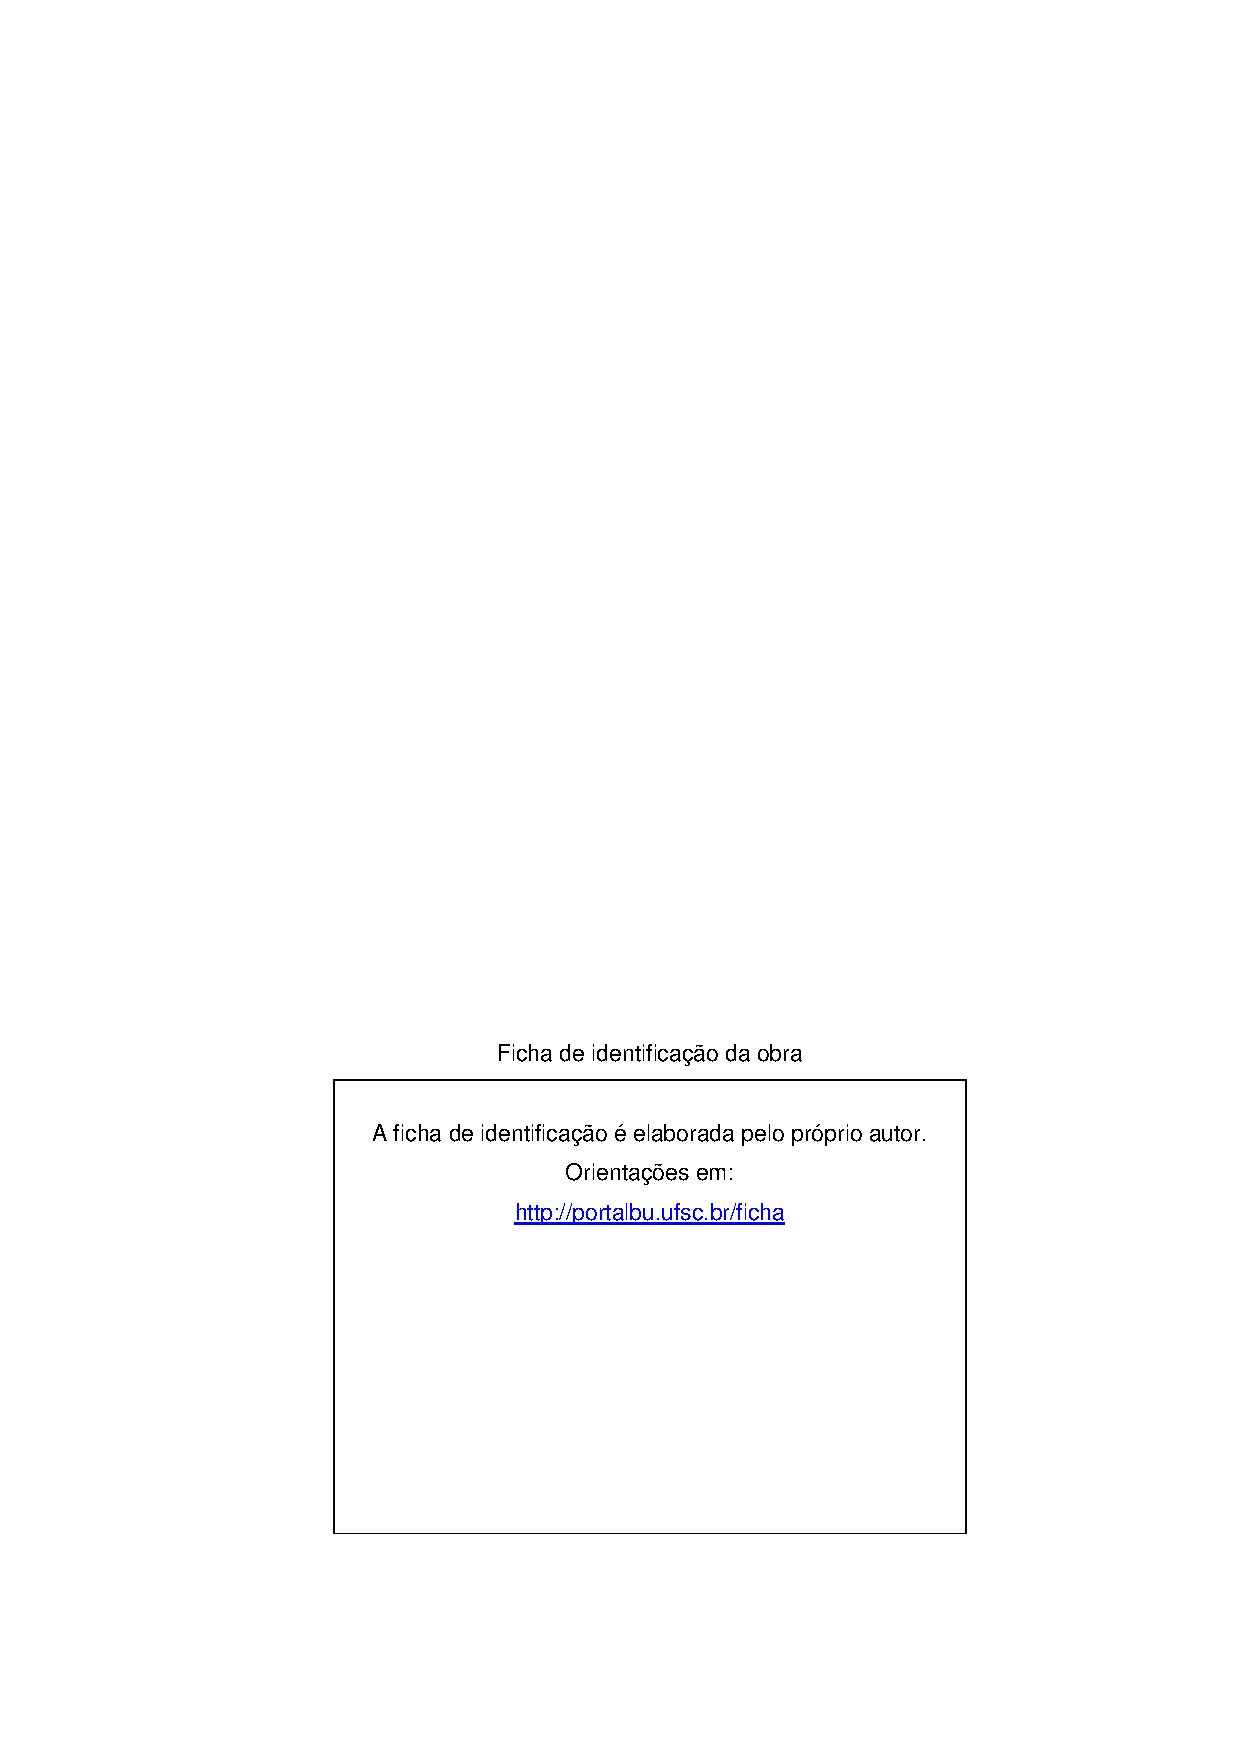
\includepdf{pictures/Ficha_Catalografica.pdf}
    \ifforcedinclude\else\cleardoublepage\fi
\fi


% Inserir errata

% Inserir folha de aprovação. Isto é um exemplo de Folha de aprovação, elemento obrigatório da
% NBR 14724/2011 (seção 4.2.1.3). Você pode utilizar este modelo até a aprovação do trabalho.
% Após isso, substitua todo o conteúdo deste arquivo por uma imagem da página assinada pela
% banca com o comando abaixo:
\ifforcedinclude\else\cleardoublepage\fi


% \addtotextpreliminarycontent{\lang{Approval Sheet}{Folha de Aprovação}}

% \begin{folhadeaprovacao}

%   \begin{center}
%     {\imprimirautor}

%     \begin{center}
%       \ABNTEXchapterfont\bfseries\MakeUppercase{\imprimirtitulo}\ifnotempty{\imprimirsubtitulo}{: \imprimirsubtitulo}
%     \end{center}

%     \begin{minipage}{\textwidth}
%       \lang
%       {
%         This \imprimirtipotrabalho~was considered appropriate to get the \imprimirformacao,
%         \ifnotempty{\imprimirarea}{in the area of \imprimirarea,}
%         and it was approved by the \imprimirprograma~of \imprimircentro~of \imprimirinstituicao.
%       }
%       {
%         Este(a) \imprimirtipotrabalho~foi julgado adequado(a) para obtenção do Título de \imprimirformacao,
%         \ifnotempty{\imprimirarea}{na área de concentração de \imprimirarea,}
%         e foi aprovado em sua forma final pelo \imprimirprograma~
%         do \imprimircentro~da \imprimirinstituicao.
%       }
%     \end{minipage}%
%   \end{center}

%   \begin{center}
%     \imprimirlocal, \imprimirdata.
%   \end{center}

%   \assinatura{%
%     \textbf{\imprimircoordenador} \\
%     \imprimircoordenadorRotulo~\lang{of}{do} \imprimirprograma
%   }

%   % \newpage
%   \begin{flushleft}
%     \textbf{\lang{Examination Board}{Banca Examinadora}:}
%   \end{flushleft}

%   \assinatura{%
%     \textbf{\imprimirorientador} \\ \imprimirorientadorRotulo\\
%     \imprimirinstituicao~--~\imprimirinstituicaosigla
%   }

%   \ifnotempty{\imprimircoorientador}{%
%     \assinatura{%
%       \textbf{\imprimircoorientador} \\ \imprimircoorientadorRotulo \\
%       \imprimirinstituicao~--~\imprimirinstituicaosigla
%     }
%   }

%   \assinatura{%
%     \textbf{Prof. Convidado 1, \lang{PhD.}{Dr.}} \\
%     Instituição 1 -- Sigla 1
%   }

%   \assinatura{%
%     \textbf{Prof. Convidado 2, \lang{PhD.}{Dr.}} \\
%     Instituição 2 -- Sigla 2
%   }

%   \assinatura{%
%     \textbf{Prof. Convidado 3, \lang{PhD.}{Dr.}} \\
%     Instituição 3 -- Sigla 3
%   }

%   \assinatura{%
%     \textbf{Prof. Convidado 4, \lang{PhD.}{Dr.}} \\
%     Instituição 4 -- Sigla 4
%   }

% \end{folhadeaprovacao}

\addtotextpreliminarycontent{\lang{Approval Sheet}{Folha de Aprovação}}

\begin{folhadeaprovacao}
  \OnehalfSpacing
  \centering
  \begin{center}
    {\imprimirautor}

    \begin{center}
      \ABNTEXchapterfont\bfseries\MakeUppercase{\imprimirtitulo}\ifnotempty{\imprimirsubtitulo}{: \imprimirsubtitulo}
    \end{center}

    \begin{minipage}{\textwidth}
      \begin{center}
        \lang
        {
          % This \imprimirtipotrabalho~was considered appropriate to get the \imprimirformacao,
          % \ifnotempty{\imprimirarea}{in the area of \imprimirarea,}
          % and it was approved by the \imprimirprograma~of \imprimircentro~of \imprimirinstituicao.
          The present \imprimirnivel~thesis was evaluated and approved by examination board formed
          by the following members:\\
        }
        {
          % Este(a) \imprimirtipotrabalho~foi julgado adequado(a) para obtenção do Título de \imprimirformacao,
          % \ifnotempty{\imprimirarea}{na área de concentração de \imprimirarea,}
          % e foi aprovado em sua forma final pelo \imprimirprograma~
          % do \imprimircentro~da \imprimirinstituicao.
          O presente trabalho em nível de \imprimirnivel~foi avaliado e
          aprovado por banca examinadora composta pelos seguintes membros:\\
        }
      \end{center}
    \end{minipage}%

    \vspace*{\baselineskip}
    \textbf{Prof. Convidado 1, \lang{PhD.}{Dr.}} \\
    Instituição 1 -- Sigla 1

    \vspace*{\baselineskip}
    \textbf{Prof. Convidado 2, \lang{PhD.}{Dr.}} \\
    Instituição 2 -- Sigla 2

    \vspace*{\baselineskip}
    \textbf{Prof. Convidado 3, \lang{PhD.}{Dr.}} \\
    Instituição 3 -- Sigla 3

    \vspace*{2\baselineskip}
    \begin{minipage}{\textwidth}
      \lang
      {
        We certify that this is the \textbf{original and final} version of this work, that was considered appropriate to get the \imprimirformacao.\\
      }
      {
        Certificamos que esta é a \textbf{versão original e final} deste trabalho, que foi julgado adequado para obtenção do título de \imprimirformacao.\\
      }
    \end{minipage}
    %    \vspace{-0.7cm}
    \vspace*{\fill}
    \assinatura{
      \OnehalfSpacing
      \textbf{\imprimircoordenador}
      \lang
      {
        Coordinator of the
      }
      {
        Coordenação do
      }
      \imprimirprograma

    }

    \vspace*{\fill}
    \assinatura{
      \OnehalfSpacing
      \textbf{\imprimirorientador} \\
      \imprimirorientadorRotulo
    }
    %	\ifnotempty{\imprimircoorientador}{
    %	\assinatura{\imprimircoorientador \\ \imprimircoorientadorRotulo \\
    %		\imprimirinstituicao~--~\imprimirinstituicaosigla}
    %	}
    % \newpage
    \vspace*{\fill}
    \imprimirlocal, \imprimirano.
  \end{center}


\end{folhadeaprovacao}
% \includepdf{pictures/folhadeaprovacao_final.pdf}


% Dedicatória
\ifforcedinclude\else\cleardoublepage\fi
\ifforcedinclude\else

\addtotextpreliminarycontent{\lang{Dedicatory}{Dedicatória}}

\begin{dedicatoria}

  \vspace*{\fill}
  \centering
  \noindent
  \textit{\lang
    {
      This work is dedicated to my grandmother Dulce Maria, \\
      and to my mother, Dulce A. Borges.
    }
    {
      Este trabalho é dedicado à minha avó Dulce Maria \\
      e à minha mãe, Dulce A. Borges..
    }
    % {
    %   This work is dedicated to adult children who, \\
    %   When small, dreamed of becoming scientists.
    % }
    % {
    %   Este trabalho é dedicado às crianças adultas que,\\
    %   quando pequenas, sonharam em se tornar cientistas.
    % }
  }
  \vspace*{\fill}

\end{dedicatoria}


\fi

% Agradecimentos
\ifforcedinclude\else\cleardoublepage\fi


\addtotextpreliminarycontent{\lang{Acknowledgement}{Agradecimentos}}

\begin{agradecimentos}

\lang
{
    Greetings.
}
{
    Os agradecimentos principais são direcionados à Gerald Weber, Miguel Frasson,
    Leslie H. Watter, Bruno Parente Lima, Flávio de Vasconcellos Corrêa, Otavio Real
    Salvador, Renato Machnievscz\footnote{Os nomes dos integrantes do primeiro
    projeto abn\TeX\ foram extraídos de
    \url{http://codigolivre.org.br/projects/abntex/}} e todos aqueles que
    contribuíram para que a produção de trabalhos acadêmicos conforme
    as normas ABNT com \LaTeX{} fosse possível.

    Agradecimentos especiais são direcionados ao Centro de Pesquisa em Arquitetura
    da Informação\footnote{\url{http://www.cpai.unb.br/}} da Universidade de
    Brasília (CPAI), ao grupo de usuários
    \emph{latex-br}\footnote{\url{http://groups.google.com/group/latex-br}} e aos
    novos voluntários do grupo
    \emph{\abnTeX{}}\footnote{\url{http://groups.google.com/group/abntex2} e
    \url{http://abntex2.googlecode.com/}}~que contribuíram e que ainda
    contribuirão para a evolução do \abnTeX{}.
}

\end{agradecimentos}


%Mesmo padrão da seção primária, porém sem indicativo numérico. Assim como: Dedicatória, Resumo, Abstract, Sumário, Listas, Referências, Apêndices e Anexos.
%
%
%Corpo do texto, fonte 10,5, justificado, recuo especial da primeira linha de 1 cm, espaçamento simples.
%


% Epígrafe
\ifforcedinclude\else\cleardoublepage\fi


\addtotextpreliminarycontent{\lang{Epigraph}{Epigrafe}}

\begin{epigrafe}

\vspace*{\fill}\lang
{
    \begin{flushright}
        \textit{``Learn from yesterday, live for today, hope for tomorrow. The important thing is not to stop questioning.''} \\ Albert Einstein
    \end{flushright}
    \begin{flushright}
        \textit{``The true sign of intelligence is not knowledge but imagination.''} \\  Albert Einstein
    \end{flushright}
    \begin{flushright}
        \textit{``Peace cannot be kept by force; it can only be achieved by understanding.''} \\ Albert Einstein
    \end{flushright}
    \begin{flushright}
        \textit{``Whoever is careless with the truth in small matters cannot be trusted with important matters.''} \\ Albert Einstein
    \end{flushright}
    \begin{flushright}
        \textit{``Extraordinary claims require extraordinary evidence''} \\ Carl Sagan
    \end{flushright}
    \begin{flushright}
        \textit{``Catholic, which I was until I reached the age of reason.''} \\ George Carlin
    \end{flushright}
    \begin{flushright}
        \textit{``We made too many wrong mistakes.''} \\ Yogi Berra
    \end{flushright}
}
{
    \begin{flushright}
        \textit{``Assim como aquele pecado da juventude, este documento te perseguirá pelo resto da vida.''} \\ Enio Valmor Kassick
    \end{flushright}
    \begin{flushright}
        \textit{``Estupidez trará mais autoconfiança do que o conhecimento e a bravura juntas. \englishword{\showfont}''} \\ Adriano Ruseler
    \end{flushright}
}

\end{epigrafe}





% Ajusta o espaçamento dos parágrafos do resumo
\setlength{\absparsep}{18pt}

% RESUMOS
\ifforcedinclude\else\cleardoublepage\fi


\newcommand{\imprimirbrazilabstract}{%
  \cleardoublepage\phantomsection
  \addtotextpreliminarycontent{Resumo em Português}
  \begin{otherlanguage*}{brazil}
    \begin{resumo}[Resumo]

      % Segundo a \textcite[3.1-3.2]{NBR6028:2003}, o resumo deve ressaltar o
      % objetivo, o método, os resultados e as conclusões do documento. A ordem e a extensão
      % destes itens dependem do tipo de resumo (informativo ou indicativo) e do
      % tratamento que cada item recebe no documento original. O resumo deve ser
      % precedido da referência do documento, com exceção do resumo inserido no
      % próprio documento. (\ldots) As palavras-chave devem figurar logo abaixo do
      % resumo, antecedidas da expressão Palavras-chave:, separadas entre si por
      % ponto e finalizadas também por ponto.

      % Além disso, na UFSC o texto do resumo deve ser digitado, em um único bloco, sem espaço de parágrafo. O resumo deve
      % ser significativo, composto de uma sequência de frases concisas, afirmativas e não de uma
      % enumeração de tópicos. Não deve conter citações. Deve usar o verbo na voz passiva. Abaixo do
      % resumo, deve-se informar as palavras-chave (palavras ou expressões significativas retiradas do
      % texto) ou, termos retirados de thesaurus da área. \englishword{\showfont}

      Deposição por energia direcionada a laser (L-DED), utilizando pó como material de adição, é uma tecnologia
      emergente na área de fabricação avançada, apresentando diversas características atraentes quando comparadas a
      outras técnicas de fabricação por manufatura aditiva de metais. Seu potencial para preencher as lacunas entre as etapas de
      desenvolvimento de produtos, prototipagem e produção de partes altamente otimizadas são notáveis, mas a complexidade
      inerente ao processo ainda levanta questionamentos relevantes que precisam ser abordados. Apesar de que
      a geometria de seções transversais de cordões individuais e paredes finas, bem como os efeitos dos parâmetros
      de processo na microestrutura resultante são amplamente discutidos na literatura para diferentes
      combinações de parâmetros e materiais processados, apenas alguns estudos investigam a formação de peças
      com características geométricas relevantes para produtos. Como o objetivo principal do processo é geralmente entregar
      componentes de boa qualidade, e a geometria final do componente desempenha um papel importante na definição de qualidade,
      o presente trabalho documenta uma abordagem inversa, investigando como características geométricas do componente
      afetam a geometria depositada resultante, para um determinado conjunto de parâmetros de processo. A espessura
      da parede, ângulo de inclinação e raio de curvatura de uma geometria paramétrica são manipulados para um
      conjunto de parâmetros de processo e as geometrias finais resultantes, bem como seções transversais locais
      são analisadas.

      \imprimirpalavraschave{Palavras-chaves}{\begin{inparaitem}[]\palavraschaveportugues\end{inparaitem}}

    \end{resumo}
  \end{otherlanguage*}
}


\newcommand{\imprimirenglishabstract}{%
  % https://tex.stackexchange.com/questions/20987/changing-babel-package-inside-a-single-chapter
  % https://tex.stackexchange.com/questions/36526/multiple-language-document-babel-selectlanguage-vs-begin-endotherlanguage
  \cleardoublepage\phantomsection
  \addtotextpreliminarycontent{English's Abstract}
  \begin{otherlanguage*}{english}
    \begin{resumo}[Abstract]

      Powder fed Laser Directed Energy Deposition (L-DED) is an emerging technology in the field
      of additive manufacturing, accounting for a variety of attractive features when compared to
      other metal additive manufacturing techniques. Its potential to fill the gaps between product
      development, prototyping and production of highly optimized parts are remarkable, but the inherent
      complexity of the process still raises relevant questions that need to be addressed. Although
      the cross-section geometry of single beads and thin walls, as well as the effects of process
      parameters on the resulting microstructure is widely discussed in the literature for different
      combinations of process parameters and materials, only a few studies investigate how bulk parts
      with product-like features are formed. As the main goal of the process is usually to deliver
      good quality parts, and the overall geometry plays a major role in the definition of quality,
      the present work takes an inverse approach, investigating how geometric features of the desired
      part affects the resulting deposited geometry, for a given set of process parameters. The wall
      thickness, draft angle and curvature radius of a benchmark geometry are manipulated for a fixed
      set of process parameters, and the resulting overall geometries, as well as local cross-sections
      are compared.

      \imprimirpalavraschave{Keywords}{\begin{inparaitem}[]\palavraschaveingles\end{inparaitem}}

    \end{resumo}
  \end{otherlanguage*}
}


% \newcommand{\imprimirfrenchabstract}{%
%     \addtotextpreliminarycontent{Français Résumé}
%     \begin{resumo}[Résumé]
%       \begin{otherlanguage*}{french}
%           Il s'agit d'un résumé en français.

%           \imprimirpalavraschave{Mots-clés}{latex. abntex. publication de textes.}
%       \end{otherlanguage*}
%     \end{resumo}
% }


% \newcommand{\imprimirspanishabstract}{%
%     \addtotextpreliminarycontent{Español Resumen}
%     \begin{resumo}[Resumen]
%       \begin{otherlanguage*}{spanish}
%           Este es el resumen en español.

%           \imprimirpalavraschave{Palabras clave}{latex. abntex. publicación de textos.}
%       \end{otherlanguage*}
%     \end{resumo}
% }


\makeatletter
\ifenglish
  \@ifundefined{imprimirbrazilabstract}{}{\imprimirbrazilabstract}

  % % https://tex.stackexchange.com/questions/331108/times-new-roman-in-latex-just-some-text
  % % https://tex.stackexchange.com/questions/11707/how-to-force-output-to-a-left-or-right-page
  % % https://tex.stackexchange.com/questions/132966/do-not-display-chapter-title-in-memoir-class
  % \cleardoublepage\phantomsection
  % \pretextualchapter{Resumo Expandido}
  % \addtotextpreliminarycontent{Resumo Expandido}

  % \begin{otherlanguage*}{brazil}
  %   \setlength{\parskip}{0.2cm}
  %   \setlength{\parindent}{0.0cm}
  %   \fontfamily{ptm}\selectfont

  %   \section*{Introdução}
  %   O resumo expandido é previsto na Resolução Normativa nº 95/CUn/2017, Art. 55, § 2, de 4 de
  %   abril de 2017, e exigido para teses e dissertações escritas em idiomas estrangeiros (com
  %   exceção dos cursos pertinentes ao estudo de idiomas estrangeiros – Programa de Pós-Graduação
  %   em Estudos da Tradução e Programa de Pós-Graduação em Inglês: Estudos Linguísticos e
  %   Literários).

  %   O resumo expandido é considerado um elemento pré-textual e deverá ser incluído no trabalho
  %   após o resumo e antes do abstract. Deverá iniciar em página impar (no anverso de uma folha)
  %   continuando no verso da folha. O texto deverá seguir o formato A5, com margens espelhadas:
  %   superior 2,0 cm, inferior 1,5 cm, interna 2,5 cm e externa 1,5. Deve ser empregada a fonte
  %   Time New Roman.  Todo o texto deve ser digitado em tamanho 10,5. O espaçamento entre as
  %   linhas deverá ser simples. A expressão “resumo expandido” deve seguir a mesma tipografia das
  %   demais sessões primárias do trabalho.

  %   O texto do resumo expandido deve ser redigido em português e conter as seguintes seções (ver
  %   modelo): Introdução, Objetivos, Metodologia, Resultados e Discussão e Considerações Finais.
  %   Deve apresentar no mínimo duas (02) e, no máximo, cinco (05) páginas contendo a mesma
  %   formatação em A5 do resumo e do abstract, bem como palavras-chave. \englishword{\showfont}

  %   \section*{Objetivos}
  %   Lorem ipsum dolor sit amet, consectetur adipiscing elit. Phasellus vitae dolor lacus. Ut
  %   accumsan vitae felis nec porttitor. Integer interdum fringilla feugiat. Nullam pulvinar sit
  %   amet tellus eget maximus. Donec sit amet magna eget justo semper fermentum vel eget velit.
  %   In iaculis imperdiet mauris, ac ornare libero placerat non. Nulla libero lectus, ullamcorper
  %   ac ornare eget, pulvinar ac nulla. Curabitur vestibulum non nisl eget sagittis. Proin
  %   gravida lacus id eros bibendum interdum. Mauris ullamcorper elementum tortor sed consequat.
  %   Integer tempus, est a lobortis vehicula, nisi mi fringilla augue, non semper leo metus in
  %   quam. Etiam in leo maximus, pulvinar mi eget, vehicula risus. Donec sed dui semper, dictum
  %   eros at, suscipit felis.

  %   Nam sagittis vel orci at tempus. Nulla non pellentesque eros.
  %   Quisque cursus leo massa, eu ultricies nisl lacinia a. Nulla sit amet elementum ligula.
  %   Proin sodales venenatis dictum. Ut et est cursus, vulputate velit et, viverra odio. Interdum
  %   et malesuada fames ac ante ipsum primis in faucibus. Maecenas purus diam, tempor a semper
  %   et, finibus a ex. Cras sagittis felis urna, et consequat arcu lacinia ut. Praesent blandit
  %   venenatis ante nec porta. Duis rutrum, tellus vitae ullamcorper auctor, lectus ex laoreet
  %   est, ac tristique ipsum arcu vitae nibh. Nam efficitur felis ut mi consectetur, nec auctor
  %   odio ornare. In tempor vulputate urna, vitae cursus enim egestas eu. Proin diam augue,
  %   dignissim vitae ligula eget, lobortis ornare odio. Duis quis elit augue. Fusce quis rhoncus
  %   tortor. Donec hendrerit at massa a mattis. Sed ipsum neque, aliquam ut sem sed, ultrices
  %   varius ligula. Suspendisse blandit, dolor ac rhoncus lacinia, dolor purus cursus purus, et
  %   accumsan orci neque a leo.

  %   \section*{Metodologia}
  %   Quisque efficitur dolor in lectus dapibus elementum. Nam ultrices blandit consectetur.
  %   Nullam ultricies sit amet odio quis placerat. Aenean eget est elit. Maecenas et nulla dolor.
  %   Orci varius natoque penatibus et magnis dis parturient montes, nascetur ridiculus mus. In
  %   pulvinar velit sed mi sagittis ornare. Aenean rutrum suscipit egestas. Phasellus pharetra
  %   eget ex in volutpat. Quisque eu arcu nunc. Vivamus arcu ligula, pharetra at rhoncus sit
  %   amet, pulvinar sed eros. Sed porta ipsum ipsum, et fermentum magna volutpat sed. Vivamus
  %   pharetra facilisis orci, sit amet luctus nisl pretium id. Sed consequat, arcu et congue
  %   pulvinar, risus enim aliquet purus, eget venenatis libero leo sit amet metus. Maecenas vitae
  %   elit sapien. Fusce mollis libero et gravida placerat. Proin ut quam quis justo aliquam
  %   dictum. Donec volutpat convallis suscipit. Vivamus metus nisl, placerat ac enim vitae,
  %   tempus ultricies odio.

  %   Aliquam ac vehicula arcu, non bibendum nulla. Morbi libero sem,
  %   imperdiet vel quam et, posuere tempus nunc. Maecenas dictum magna sit amet ligula facilisis
  %   commodo. Aliquam tellus diam, ornare vel elementum in, dignissim id purus. Ut at tortor non
  %   sem molestie euismod non at turpis. Phasellus vitae bibendum tellus. Suspendisse odio enim,
  %   faucibus eget congue quis, semper sit amet tortor. Sed ac lectus est. Pellentesque nec
  %   mattis mi, et varius dolor. Aliquam quis massa ac tellus malesuada sollicitudin. Maecenas
  %   ultrices risus massa, nec auctor risus sagittis id. Praesent a sapien nulla. Donec
  %   tincidunt, metus quis hendrerit facilisis, enim augue convallis elit, sed consequat lacus
  %   odio vitae magna.

  %   \section*{Resultados e Discussão}
  %   Nullam sed cursus leo. Donec commodo volutpat hendrerit. Fusce et tempus lectus, feugiat
  %   consequat est. Class aptent taciti sociosqu ad litora torquent per conubia nostra, per
  %   inceptos himenaeos. Nam quis cursus mauris, non tempus orci. Phasellus lobortis et mauris at
  %   vulputate. Sed nec nisl elementum lorem commodo gravida non a enim. Phasellus neque erat,
  %   aliquet ac ligula ac, maximus vestibulum sem. Vestibulum vel tincidunt turpis. Donec lacinia
  %   rutrum dolor dapibus bibendum. Mauris pharetra nibh nec tincidunt iaculis. Vivamus pharetra
  %   bibendum nisl eget blandit. In lobortis diam non justo eleifend, id lobortis ante fringilla.
  %   Donec libero tortor, suscipit vestibulum vestibulum id, rutrum accumsan turpis. Phasellus
  %   sollicitudin luctus tincidunt. Suspendisse potenti. Nam semper metus et mi pharetra, in
  %   pretium ligula fermentum. Integer consectetur, orci non placerat feugiat, dui ex gravida
  %   augue, vel placerat ligula augue vel velit. Aliquam sollicitudin pellentesque congue. Donec
  %   vitae turpis in ante posuere posuere. Pellentesque eu justo leo. Donec quis elit vitae leo
  %   varius luctus quis eget justo.

  %   Vestibulum elementum ex neque, quis commodo tortor porttitor
  %   mattis. Mauris vel sagittis turpis. Aenean ligula turpis, eleifend at felis sed, cursus
  %   condimentum orci. Fusce accumsan est odio, eu venenatis massa sodales in. Curabitur a tempor
  %   nisl. Quisque consequat sed arcu a congue. In viverra, ex ut hendrerit condimentum, urna sem
  %   euismod eros, nec suscipit turpis dolor eget augue. Aenean posuere tellus et consectetur
  %   condimentum. Mauris et massa et nulla fringilla interdum. Duis quis posuere elit. Donec at
  %   ex non arcu faucibus rutrum et vel lectus. Vivamus pellentesque vestibulum rutrum. Sed
  %   pretium, purus sed efficitur feugiat, nisi justo eleifend nibh, id suscipit nunc massa nec
  %   lectus. In euismod enim eu sapien dictum sodales. Fusce sit amet vulputate orci. Nulla
  %   rutrum mauris at purus aliquet, ac sollicitudin leo laoreet. Etiam elementum posuere
  %   feugiat. Maecenas sed libero non augue fermentum ultricies eget at mi. Aenean auctor
  %   bibendum lacus, dignissim aliquet est tempus eget. Maecenas tempus, nulla id rhoncus
  %   suscipit, augue leo auctor mi, eget tincidunt magna mi quis dui. Maecenas ut elit in turpis
  %   tincidunt ultrices. Nulla id nulla aliquet, porttitor eros quis, egestas justo. Nunc nisi
  %   quam, egestas a accumsan fermentum, ultricies ac elit.

  %   Nulla porta auctor vestibulum. Sed
  %   consectetur lacus molestie iaculis ullamcorper. Proin porta posuere massa a lacinia. Nunc a
  %   lacinia orci, non vehicula ante. Vestibulum ipsum velit, congue et neque aliquam, imperdiet
  %   ornare augue. Donec et congue sapien. Pellentesque consequat consectetur neque ut varius. In
  %   aliquam ex quis ante venenatis dapibus. Vivamus et imperdiet urna. Vestibulum quis nibh
  %   magna. In a congue lectus, eu sodales nunc. Suspendisse id.

  %   \section*{Considerações Finais}
  %   Lorem ipsum dolor sit amet, consectetur adipiscing elit. Phasellus vitae dolor lacus. Ut
  %   accumsan vitae felis nec porttitor. Integer interdum fringilla feugiat. Nullam pulvinar sit
  %   amet tellus eget maximus. Donec sit amet magna eget justo semper fermentum vel eget velit.
  %   In iaculis imperdiet mauris, ac ornare libero placerat non. Nulla libero lectus, ullamcorper
  %   ac ornare eget, pulvinar ac nulla. Curabitur vestibulum non nisl eget sagittis. Proin
  %   gravida lacus id eros bibendum interdum. Mauris ullamcorper elementum tortor sed consequat.
  %   Integer tempus, est a lobortis vehicula, nisi mi fringilla augue, non semper leo metus in
  %   quam. Etiam in leo maximus, pulvinar mi eget, vehicula risus. Donec sed dui semper, dictum
  %   eros at, suscipit felis.

  %   Nam sagittis vel orci at tempus. Nulla non pellentesque eros.
  %   Quisque cursus leo massa, eu ultricies nisl lacinia a. Nulla sit amet elementum ligula.
  %   Proin sodales venenatis dictum. Ut et est cursus, vulputate velit et, viverra odio. Interdum
  %   et malesuada fames ac ante ipsum primis in faucibus. Maecenas purus diam, tempor a semper
  %   et, finibus a ex. Cras sagittis felis urna, et consequat arcu lacinia ut. Praesent blandit
  %   venenatis ante nec porta. Duis rutrum, tellus vitae ullamcorper auctor, lectus ex laoreet
  %   est, ac tristique ipsum arcu vitae nibh. Nam efficitur felis ut mi consectetur, nec auctor
  %   odio ornare. In tempor vulputate urna, vitae cursus enim egestas eu. Proin diam augue,
  %   dignissim vitae ligula eget, lobortis ornare odio. Duis quis elit augue. Fusce quis rhoncus
  %   tortor. Donec hendrerit at massa a mattis. Sed ipsum neque, aliquam ut sem sed, ultrices
  %   varius ligula. Suspendisse blandit, dolor ac rhoncus lacinia, dolor purus cursus purus, et
  %   accumsan orci neque a leo.


  %   \imprimirpalavraschave{Palavras-chaves}{\begin{inparaitem}[]\palavraschaveportugues\end{inparaitem}}

  % \end{otherlanguage*}

  \@ifundefined{imprimirenglishabstract}{}{\imprimirenglishabstract}

\else
  \@ifundefined{imprimirbrazilabstract}{}{\imprimirbrazilabstract}
  \@ifundefined{imprimirenglishabstract}{}{\imprimirenglishabstract}
\fi

\@ifundefined{imprimirfrenchabstract}{}{\imprimirfrenchabstract}
\@ifundefined{imprimirspanishabstract}{}{\imprimirspanishabstract}
\makeatother



% Some tables of contents
\ifforcedinclude\else
{
    % https://tex.stackexchange.com/questions/179506/disable-colorlinks-locally-or-just-for-the-toc
    \hypersetup{hidelinks}

    % inserir lista de figuras
    \ifforcedinclude\else\cleardoublepage\fi
    % https://tex.stackexchange.com/questions/234398/list-of-figures-and-tables-when-there-are-no-figures-or-tables
    \whenlistisnotempty{\listfigurename}{%
        \addtotextpreliminarycontent{\listfigurename}
        % https://tex.stackexchange.com/questions/121879/remove-spacing-between-per-chapter-figures-in-lof
        {\renewcommand{\addvspace}[1]{}
        \listoffigures*}
    }{\pdfbookmark[0]{\listfigurename}{lof}}

    % inserir lista de quadros
    \ifforcedinclude\else\cleardoublepage\fi
    % https://tex.stackexchange.com/questions/234398/list-of-figures-and-tables-when-there-are-no-figures-or-tables
    \whenlistisnotempty{\listofquadrosname}{%
        \addtotextpreliminarycontent{\listofquadrosname}
        % https://tex.stackexchange.com/questions/121879/remove-spacing-between-per-chapter-figures-in-lof
        {\renewcommand{\addvspace}[1]{}
        \listofquadros*}
    }{\pdfbookmark[0]{\listofquadrosname}{loq}}

    % inserir lista de tabelas
    \ifforcedinclude\else\cleardoublepage\fi
    % https://tex.stackexchange.com/questions/234398/list-of-figures-and-tables-when-there-are-no-figures-or-tables
    \whenlistisnotempty{\listtablename}{%
        \addtotextpreliminarycontent{\listtablename}
        % https://tex.stackexchange.com/questions/121879/remove-spacing-between-per-chapter-figures-in-lof
        {\renewcommand{\addvspace}[1]{}
        \listoftables*}
    }{\pdfbookmark[0]{\listtablename}{lot}}

    % inserir códigos fonte (List of Listings `lol`)
    % https://tex.stackexchange.com/questions/511519/latex-keeps-showing-minted-environment-as-figures-instead-of-listening/511579#511579
    \ifforcedinclude\else\cleardoublepage\fi
    % https://tex.stackexchange.com/questions/234398/list-of-figures-and-tables-when-there-are-no-figures-or-tables
    \whenlistisnotempty{\lstlistlistingname}{%
        \addtotextpreliminarycontent{\lstlistlistingname}
        % https://tex.stackexchange.com/questions/121879/remove-spacing-between-per-chapter-figures-in-lof
        {\renewcommand{\addvspace}[1]{}
        \lstlistoflistings*}
    }{\pdfbookmark[0]{\lstlistlistingname}{lol}}
}
\fi


% inserir lista de abreviaturas e siglas
\ifforcedinclude\else\cleardoublepage\fi


\addtotextpreliminarycontent{\lang{List of Acronyms}{Lista de Siglas}}

\begin{siglas}
    \item[ABNT] \lang{Brazilian Association of Technical Standards}{Associação Brasileira de Normas Técnicas}
    \item[abnTeX] \lang{Absurd Standards for TeX}{ABsurdas Normas para TeX}
\end{siglas}



% Inserir lista de símbolos
\ifforcedinclude\else\cleardoublepage\fi


\addtotextpreliminarycontent{\lang{List of Symbols}{Lista de Símbolos}}

% Devam aparecer na mesma ordem de ocorrência no texto.
\begin{simbolos}
    \item[$ \Gamma $] \lang{Greek letter Gama}{Letra grega Gama}
    \item[$ \Lambda $] \lang{Lambda}{Lambda}
    \item[$ \zeta $] \lang{Minimal Greek letter zeta}{Letra grega minúscula zeta}
    \item[$ \in $] \lang{Belongs}{Pertence}
\end{simbolos}


% How to remove the self-reference of the ToC from the ToC?
% https://tex.stackexchange.com/questions/10943/how-to-remove-the-self-reference-of-the-toc-from-the-toc
\ifforcedinclude\else\cleardoublepage\fi

\begin{KeepFromToc}
    % https://tex.stackexchange.com/questions/35/what-does-overfull-hbox-mean
    % https://tex.stackexchange.com/questions/59122/how-to-avoid-using-sloppy-document-wide-to-fix-overfull-hbox-problems
    % https://tex.stackexchange.com/questions/257007/adding-color-to-table-of-contents-and-section-headings
    {
        % https://tex.stackexchange.com/questions/179506/disable-colorlinks-locally-or-just-for-the-toc
        \hypersetup{hidelinks}

        % https://tex.stackexchange.com/questions/65711/underfull-vbox-badness-10000-with-memoir
        \raggedbottom

        % https://tex.stackexchange.com/questions/49887/overfull-hbox-warning-for-toc-entries-when-using-memoir-documentclass
        % \makeatletter
            % \renewcommand{\@pnumwidth}{2em}
            % \renewcommand{\@tocrmarg}{3em}
        % \makeatother

        % https://tex.stackexchange.com/questions/57544/memoir-mysterious-overfull-hbox-in-toc-when-mathptmx-is-used
        % \setlength{\cftchapternumwidth}{2.25em}

        % Add the table of contents to the brief table of contents
        % https://tex.stackexchange.com/questions/234398/list-of-figures-and-tables-when-there-are-no-figures-or-tables
        \whenlistisnotempty{\contentsname}{%
            \addtotextpreliminarycontent{\contentsname}
            \tableofcontents
        }{\pdfbookmark[0]{\contentsname}{toc}}
    }

\end{KeepFromToc}



% ELEMENTOS TEXTUAIS
\textual
\setlength\beforechapskip{50pt}
\setlength\midchapskip{20pt}
\setlength\afterchapskip{20pt}

% PARTE
\ifforcedinclude\else\part{\lang{Research}{Pesquisa}}\fi
\label{primeira_parte}

% Introdução (exemplo de capítulo sem numeração, mas presente no Sumário)
% The \phantomsection command is needed to create a link to a place in the document that is not a
% figure, equation, table, section, subsection, chapter, etc.
% https://tex.stackexchange.com/questions/44088/when-do-i-need-to-invoke-phantomsection
\phantomsection

% https://tex.stackexchange.com/questions/5076/is-it-possible-to-keep-my-translation-together-with-original-text
\chapter{\lang{Introduction}{Introdução}}
\phantomsection

{\lang{
    Additive manufacturing (AM) has gained attention for the last two decades for its great potential
    to reduce the time between ideation and production of complex geometries. This characteristic is
    being frequently explored among researchers and engineers to evaluate and compare product concepts
    beyond virtual models and prior to investing in tooling for mass production. The reduced supply
    chain, also has an enormous potential to decrease the lead time between a sales order and the
    delivery of a functional component, consequently reducing inventory cost \cite{VOLPATO2017}.
  }
  {}
}

{\lang{
    Other great potentials of the technology are the reduction of geometric constraints, removing
    barriers to the production of components optimized for multi-physics restrictions and the possibility
    to repair components. These characteristics combined can result in lower assembly part count and
    component weight, as well as cheaper maintenance, leading to lifetime cost reduction, more efficient
    operation and less fuel consumption in systems such as airplanes \cite{ZHANG2017148}.
    \autoref{fig_ma_examples} illustrates applications of different AM technologies used in the aerospace industry.
  }
  {}
}

\begin{figure}[htb]
  \caption{
    \lang{
      Examples of additive manufacturing of metallic components. (a) LBM-produced Ti-6Al-4V bracket
      for Airbus A350 with topology optimized bionic design resulting in ~30 weight saving cp.
      to conventional milled bracket \cite{LIU2017351}. (b) Turbine housing fabricated by the LASERTEC
      65 3D System using multi-axis deposition. (c) Exhaust duct fabricated using the Laser Engineered
      Net Shape (LENS) process \cite{LIU2017351}. (d) Repairing for damaged titanium blisk \cite{SABOORIetAll2019}.
    }{
      Exemplos de manufatura aditiva de componentes metálicos
    }
  }  \label{fig_ma_examples}
  \centering
  \begin{subfigure}{0.24\textwidth}
    \label{fig_ma_examples_a}
    \centering
    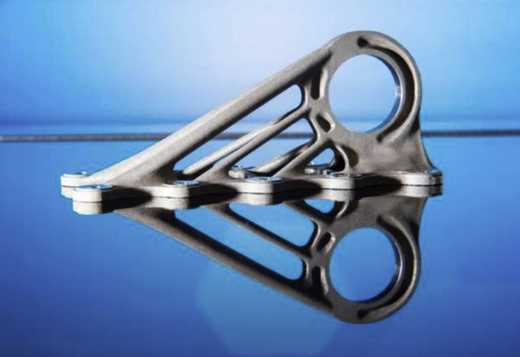
\includegraphics[width=\textwidth]{airbus_bracket_a.png}
    \caption{}
  \end{subfigure}
  \hfill
  \begin{subfigure}{0.24\textwidth}
    \label{fig_ma_examples_b}
    \centering
    \adjincludegraphics[trim=0 {.38\height} 0 0,clip,width=\textwidth]{turbine_housing_b.png}
    \caption{}
  \end{subfigure}
  \hfill
  \begin{subfigure}{0.24\textwidth}
    \label{fig_ma_examples_c}
    \centering
    \adjincludegraphics[trim=0 0 0 {.25\height},clip,width=\textwidth]{exhaust_duct_c.png}
    \caption{}
  \end{subfigure}
  \hfill
  \begin{subfigure}{0.24\textwidth}
    \label{fig_ma_examples_d}
    \centering
    \adjincludegraphics[trim=0 {.15\height} 0 {.15\height},clip,width=\textwidth]{titanium_blisk_repair_d.png}
    \caption{}
  \end{subfigure}
  \hfill

\end{figure}

{\lang{
  Despite the promising features, AM is still expensive when compared to other manufacturing processes,
  especially for processing metals, with only a few technologies applicable to manufacture dense
  components. To accomplish that, Powder Bed Fusion (PBF), Sheet Lamination (SL) and Directed Energy
  Deposition (DED) are some of the AM groups of process available, each one presenting particular
  strengths and limitations \cite{VOLPATO2017}.
}
{}
}

{\lang{
  Among the above mentioned categories, Directed Energy Deposition Laser with Powder as feedstock
  material (DED-LP), a sub category of DED processes, offers advantages such as suitability to repair
  failed components, suitability to produce larger parts with higher build rates when compared to PBF
  technology and the potential to manufacture components with variations in alloy composition along
  the build volume, an advanced class of materials known as Functionally Graded Materials (FGM) \cite{VOLPATO2017}
  \cite{DEBROYetAll2018112}. On the other hand PBF technology offer much better geometry resolution,
  design freedom and enhanced mechanical properties, being one of the most widespread metal manufacturing
  processes \cite{LEWANDOWSKIandSEIFI2016}\cite{FRAZIER2014}.
}
{}
}

{\lang{
  Although some authors argue that the production cost will drop as technology evolves, manufacturing
  metal components by AM is still only justifiable when a significant reduction in lead time, inventory
  cost, part weight or part count takes place \cite{BOURELLetAl2009}. Furthermore, the lack of diffuse
  knowledge of process dependent geometry limitations and output material properties, restrict the choice
  of manufacturing process according to the availability of material data still in the design phase
  \cite{ASHBY2011xi}.
}
{}
}

{\lang{
  In this context, the mechanical properties resulting from the process are of special interest given
  the fact that metals are extensively used to withstand the mechanical loads of a variety of
  applications. Information extracted from stress-strain curves such as Young’s modulus (E), elastic
  limit (Sy) and tensile strength (Su) are the baseline information for the mechanical design of
  structural components as illustrates \autoref{fig_material_information}.
}
{}
}


\begin{figure}[htb]
  \caption{
    \lang{
      Types of material information. Structured data for design “allowables” and the characteristics
      of a material that relate to its ability to be formed, joined, and finished; records of experience
      with its use; and design guidelines for its use \cite{ASHBY2011xi}.
    }{
      Tipos de informação do material.
    }
  }  \label{fig_material_information}
  \centering
  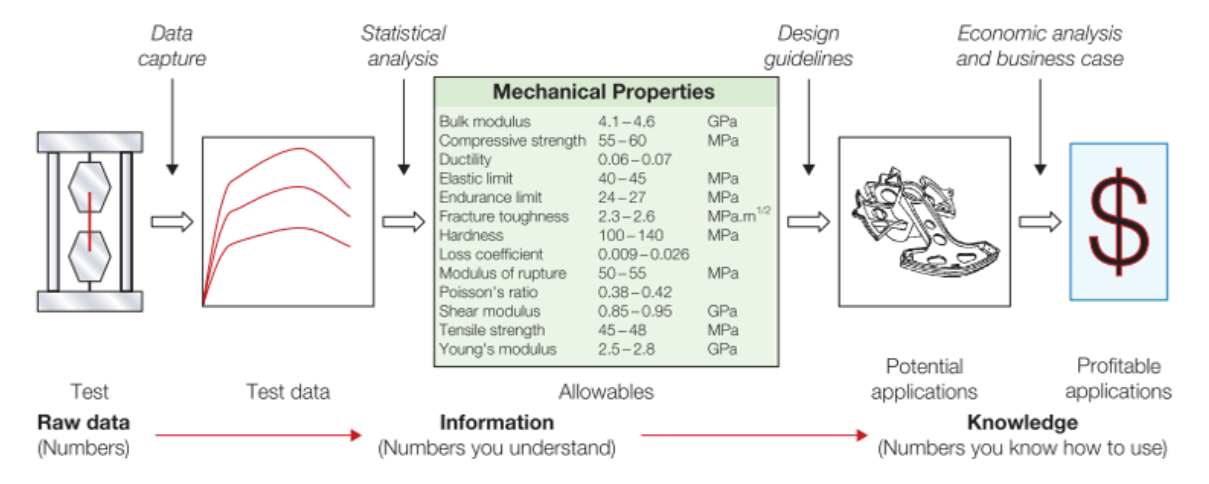
\includegraphics[width=\textwidth]{types_of_material_information.png}
\end{figure}

{\lang{
  Even though an enormous effort has been made for the last decade in order to standardize manufacturing
  practices and data reporting on mechanical properties, a collective understanding of the AM design
  paradigm as well as a database of material properties for different processing conditions is still
  required in order to democratize the technology \cite{BOURELLetAl2014}\cite{BOURELLetAl2009}.
}
{}
}




% Capitulo com exemplos de comandos inseridos de arquivo externo
%% chapters/chapter_1.tex
%%
%% Copyright 2017 Evandro Coan
%% Copyright 2012-2014 by abnTeX2 group at http://abntex2.googlecode.com/
%%
%% This work may be distributed and/or modified under the
%% conditions of the LaTeX Project Public License, either version 1.3
%% of this license or (at your option) any later version.
%% The latest version of this license is in
%%   http://www.latex-project.org/lppl.txt
%% and version 1.3 or later is part of all distributions of LaTeX
%% version 2005/12/01 or later.
%%
%% This work has the LPPL maintenance status `maintained'.
%%
%% The Current Maintainer of this work is the Evandro Coan.
%%
%% The last Maintainer of this work was the abnTeX2 team, led
%% by Lauro César Araujo. Further information are available on
%% https://www.abntex.net.br/
%%
%% This work consists of a bunch of files. But originally there were 2 files
%% which are renamed as follows:
%% Deleted the `abntex2-modelo-img-marca.pdf`
%% Renamed the `abntex2-modelo-include-comandos.tex, v-1.9.2 laurocesar` to `chapters/chapter_1.tex`
%%
% ---
% Este capítulo, utilizado por diferentes exemplos do abnTeX2, ilustra o uso de
% comandos do abnTeX2 e de LaTeX.
% ---

% The \phantomsection command is needed to create a link to a place in the document that is not a
% figure, equation, table, section, subsection, chapter, etc.
% https://tex.stackexchange.com/questions/44088/when-do-i-need-to-invoke-phantomsection
\phantomsection

% https://tex.stackexchange.com/questions/5076/is-it-possible-to-keep-my-translation-together-with-original-text
\chapter[\lang{Abbreviation for the Table of Contents}{Abreviação para o Sumário}]
{
    \lang
    {Long title to present in the chapter, Axioms, Theorems, Postulates, corollaries, lemmas}
    {Longo título apresentar no capítulo, Axiomas, Teoremas, Postulados, corolários, lemas}
}

\label{cap_exemplos}


\begin{flushright}
    \englishword{\showfont}
\end{flushright}

% Why latex is letting my text goes out of the screen?
% https://tex.stackexchange.com/questions/386762/why-latex-is-letting-my-text-goes-out-of-the-screen
\sloppy
\textbf{textbf: \englishword{\showfont}}
\fussy



\section{Axiomas ou postulados}

Na lógica tradicional, um axioma ou postulado é uma sentença ou proposição que não é provada ou demonstrada e é considerada como óbvia ou como um consenso inicial necessário para a construção ou aceitação de uma teoria. Por essa razão, é aceito como verdade e serve como ponto inicial para dedução e inferências de outras verdades (dependentes de teoria). -- \showfont


Na matemática, um axioma é uma hipótese inicial de qual outros enunciados são logicamente derivados. Pode ser uma sentença, uma proposição, um enunciado ou uma regra que permite a construção de um sistema formal. Diferentemente de teoremas, axiomas não podem ser derivados por princípios de dedução e nem são demonstráveis por derivações formais, simplesmente porque eles são hipóteses iniciais. Isto é, não há mais nada a partir do que eles seguem logicamente (em caso contrário eles seriam chamados teoremas). Em muitos contextos, "axioma", "postulado" e "hipótese" são usados como sinônimos. -- \showfont


\begin{axioma}[Axioma de Igualdade -- \showfont]
Supondo $\mathfrak{L}$, uma linguagem de primeira ordem. para cada variável $x$, a fórmula $x = x$ é universalmente válida. -- \showfont
\end{axioma}


\begin{postulado}[Postulado de Igualdade -- \showfont]
    Supondo $\mathfrak{L}$, uma linguagem de primeira ordem. para cada variável $x$, a fórmula $x = x$ é universalmente válida. -- \showfont
\end{postulado}


\section{Teorema}

Na matemática, um teorema é uma afirmação que pode ser provada como verdadeira através de outras afirmações já demonstradas, como outros teoremas, juntamente com afirmações anteriormente aceitas, como axiomas. Prova é o processo de mostrar que um teorema está correto. O termo teorema foi introduzido por Euclides, em Elementos, para significar "afirmação que pode ser provada". Em grego, originalmente significava "espetáculo" ou "festa". Atualmente, é mais comum deixar o termo "teorema" apenas para certas afirmações que podem ser provadas e de grande "importância matemática", o que torna a definição um tanto subjetiva.

\begin{teorema}[Teorema de Pitágoras -- \showfont]
    Em qualquer triângulo retângulo, o quadrado do comprimento da hipotenusa é igual à soma dos quadrados dos comprimentos dos catetos -- \showfont.
\end{teorema}


\begin{proposicao}
Em qualquer proposição a hipótese é considerada verdadeira. -- \showfont
\end{proposicao}


\subsection{Terminologia}

Usualmente deixa-se o termo ``teorema'' apenas para as afirmações que podem ser provadas de grande importância. Assim, são dados outros nomes para os outros tipos dessas afirmações -- \showfont:

\begin{description}
    \item[Proposição:] Uma Proposição é uma sentença não associada a algum outro teorema, de simples prova e de importância matemática menor -- \showfont.
    \item[Lema:] Um Lema é um ``pré-teorema'', um teorema que serve para ajudar na prova de outro teorema maior. A distinção entre teoremas e lemas é um tanto quanto arbitrária, uma vez que grandes resultados são usados para provar outros. Por exemplo, o Lema de Gauss e o Lema de Zorn são muito interessantes de per se, e muitos autores os denominam de Lemas, mesmo que não os usem para provar alguma outra coisa. -- \showfont
    \item[Corolário:] Um Corolário é uma consequência direta de outro teorema ou de uma definição, muitas vezes tendo suas demonstrações omitidas, por serem simples. -- \showfont
\end{description}


\begin{corolario}
    Em qualquer triângulo retângulo, a hipotenusa é maior que qualquer um dos catetos, mas menor que a soma deles. -- \showfont
\end{corolario}

Alguns outros termos também são usados, por mais que raros e com definição menos rigorosa, basicamente sendo usadas quando não se quer usar a a palavra ``teorema'' -- \showfont:

Regra.
Lei, que também pode se referir a axiomas, regras de dedução e a distribuições de Probabilidade.
Princípio.
Algoritmo (como em Algoritmo da Divisão), muito raro e diferente do conceito com o mesmo nome que é um dos estudos centrais da Ciência da Computação.
Paradoxo, usado quando a afirmação vai aparentemente de encontro com alguma outra verdade ou com alguma noção intuitiva. Entretanto, tal termo também pode ser usado para afirmações falsas que aparentem ser verdadeiras em um primeiro momento. -- \showfont

Alguns teoremas continuam a ser chamados de Conjecturas logo após serem provados (por exemplo, a Conjectura de Poincaré). O termo conjectura é usado para afirmações que não se sabe se são verdadeiras, e que acredita-se que são verdadeiras, mas nunca ninguém conseguiu prová-las nem negá-las (às vezes conjecturas são chamadas de hipóteses (como em Hipótese de Riemann), obviamente, num sentido diferente do aqui já descrito). -- \showfont


\subsection{Conjectura ou hipótese}

Uma conjectura é uma ideia, fórmula ou frase, a qual não foi provada ser verdadeira, baseada em suposições ou ideias com fundamento não verificado. As conjecturas utilizadas como prova de resultados matemáticos recebem o nome de hipóteses. -- \showfont



\begin{conjectura}[Conjectura dos primos gêmeos -- \showfont]
Existem infinitos números primos gêmeos. -- \showfont
\end{conjectura}

Um par de primos é chamado de primos gêmeos se eles são dois números primos $p$, $q$ tais que $q = p + 2$. -- \showfont



\subsection{Lema}

    Na Matemática, um lema é um teorema que é usado como um passo intermediário para atingir um resultado maior, provado em outro teorema. Normalmente o lema tem pouca serventia além de servir ao propósito do teorema que o utiliza, mas isto não é uma regra, e a classificação entre lemas e teoremas é arbitrária\footnote{Wikipédia -- \showfont} -- \showfont.



% https://tex.stackexchange.com/questions/20987/changing-babel-package-inside-a-single-chapter
\begin{otherlanguage*}{english}

\begin{lema}
    Given two line segments whose lengths are $a$ and $b$ respectively there is a
    real number $r$ such that $b=ra$. -- \showfont
\end{lema}



Unnumbered theorem-like environments are also possible -- \showfont.

\begin{observacao}
    This statement is true, I guess. -- \showfont
\end{observacao}

And the next is a somewhat informal definition. -- \showfont


\begin{definicao}[Fibration -- \showfont]
    A fibration is a mapping between two topological spaces that has the homotopy lifting property for every space $X$. -- \showfont
\end{definicao}

\begin{exemplo}[Fibration -- \showfont]
    A fibration is a mapping between two topological spaces that has the homotopy lifting property for every space $X$. -- \showfont
\end{exemplo}


\begin{exercicio}
    Este é um exercício -- \showfont

\end{exercicio}


\begin{exercicio}
    Mais um exercício para vocês... -- \showfont

\end{exercicio}


\begin{condicao}[Fibration -- \showfont]
    A fibration is a mapping between two topological spaces that has the homotopy lifting property for every space $X$. -- \showfont
\end{condicao}
Theorem styles

\begin{description}
    \item[definition] boldface title, romand body. Commonly used in definitions, conditions, problems and examples. -- \showfont
\item[plain] boldface title, italicized body. Commonly used in theorems, lemmas, corollaries, propositions and conjectures.
\item[remark] italicized title, romman body. Commonly used in remarks, notes, annotations, claims, cases, acknowledgments and conclusions.
\end{description}

\end{otherlanguage*}



\section{Rotação de equações}

trecho de código para rotacionar e reduzir a fonte de equações. -- \showfont

\begin{verbatim}
\begin{sideways}%
  \parbox{1\textheight}{%
      \begin{tiny}
          \begin{equation}

          \end{equation}
      \end{tiny}}
\end{sideways}
\end{verbatim}


Segue um exemplo de rotação de páginas -- \showfont: \newpage

\begin{sideways}%
    \parbox{1\textheight}{%
        \begin{tiny}
\begin{equation}
\left[ {{L_{sr}}} \right] = \left[ {\begin{array}{*{20}{c}}
    {\cos \left( \theta  \right)}&{\cos \left( {\theta  - 8\alpha } \right)}&{\cos \left( {\theta  - 7\alpha } \right)}&{\cos \left( {\theta  - 6\alpha } \right)}&{\cos \left( {\theta  - 5\alpha } \right)}&{\cos \left( {\theta  - 4\alpha } \right)}&{\cos \left( {\theta  - 3\alpha } \right)}&{\cos \left( {\theta  - 2\alpha } \right)}&{\cos \left( {\theta  - \alpha } \right)}\\
    {\cos \left( {\theta  - \alpha } \right)}&{\cos \left( \theta  \right)}&{\cos \left( {\theta  - 8\alpha } \right)}&{\cos \left( {\theta  - 7\alpha } \right)}&{\cos \left( {\theta  - 6\alpha } \right)}&{\cos \left( {\theta  - 5\alpha } \right)}&{\cos \left( {\theta  - 4\alpha } \right)}&{\cos \left( {\theta  - 3\alpha } \right)}&{\cos \left( {\theta  - 2\alpha } \right)}\\
    {\cos \left( {\theta  - 2\alpha } \right)}&{\cos \left( {\theta  - \alpha } \right)}&{\cos \left( \theta  \right)}&{\cos \left( {\theta  - 8\alpha } \right)}&{\cos \left( {\theta  - 7\alpha } \right)}&{\cos \left( {\theta  - 6\alpha } \right)}&{\cos \left( {\theta  - 5\alpha } \right)}&{\cos \left( {\theta  - 4\alpha } \right)}&{\cos \left( {\theta  - 3\alpha } \right)}\\
    {\cos \left( {\theta  - 3\alpha } \right)}&{\cos \left( {\theta  - 2\alpha } \right)}&{\cos \left( {\theta  - \alpha } \right)}&{\cos \left( \theta  \right)}&{\cos \left( {\theta  - 8\alpha } \right)}&{\cos \left( {\theta  - 7\alpha } \right)}&{\cos \left( {\theta  - 6\alpha } \right)}&{\cos \left( {\theta  - 5\alpha } \right)}&{\cos \left( {\theta  - 4\alpha } \right)}\\
    {\cos \left( {\theta  - 4\alpha } \right)}&{\cos \left( {\theta  - 3\alpha } \right)}&{\cos \left( {\theta  - 2\alpha } \right)}&{\cos \left( {\theta  - \alpha } \right)}&{\cos \left( \theta  \right)}&{\cos \left( {\theta  - 8\alpha } \right)}&{\cos \left( {\theta  - 7\alpha } \right)}&{\cos \left( {\theta  - 6\alpha } \right)}&{\cos \left( {\theta  - 5\alpha } \right)}\\
    {\cos \left( {\theta  - 5\alpha } \right)}&{\cos \left( {\theta  - 4\alpha } \right)}&{\cos \left( {\theta  - 3\alpha } \right)}&{\cos \left( {\theta  - 2\alpha } \right)}&{\cos \left( {\theta  - \alpha } \right)}&{\cos \left( \theta  \right)}&{\cos \left( {\theta  - 8\alpha } \right)}&{\cos \left( {\theta  - 7\alpha } \right)}&{\cos \left( {\theta  - 6\alpha } \right)}\\
    {\cos \left( {\theta  - 6\alpha } \right)}&{\cos \left( {\theta  - 5\alpha } \right)}&{\cos \left( {\theta  - 4\alpha } \right)}&{\cos \left( {\theta  - 3\alpha } \right)}&{\cos \left( {\theta  - 2\alpha } \right)}&{\cos \left( {\theta  - \alpha } \right)}&{\cos \left( \theta  \right)}&{\cos \left( {\theta  - 8\alpha } \right)}&{\cos \left( {\theta  - 7\alpha } \right)}\\
    {\cos \left( {\theta  - 7\alpha } \right)}&{\cos \left( {\theta  - 6\alpha } \right)}&{\cos \left( {\theta  - 5\alpha } \right)}&{\cos \left( {\theta  - 4\alpha } \right)}&{\cos \left( {\theta  - 3\alpha } \right)}&{\cos \left( {\theta  - 2\alpha } \right)}&{\cos \left( {\theta  - \alpha } \right)}&{\cos \left( \theta  \right)}&{\cos \left( {\theta  - 8\alpha } \right)}\\
    {\cos \left( {\theta  - 8\alpha } \right)}&{\cos \left( {\theta  - 7\alpha } \right)}&{\cos \left( {\theta  - 6\alpha } \right)}&{\cos \left( {\theta  - 5\alpha } \right)}&{\cos \left( {\theta  - 4\alpha } \right)}&{\cos \left( {\theta  - 3\alpha } \right)}&{\cos \left( {\theta  - 2\alpha } \right)}&{\cos \left( {\theta  - \alpha } \right)}&{\cos \left( \theta  \right)}
    \end{array}} \right]
\end{equation}
\end{tiny}
}
\end{sideways}


\begin{landscape}

Outra forma é utilizar o pacote pdflscape -- \showfont

% https://tex.stackexchange.com/questions/60453/reducing-font-size-in-equation
\tiny -- \showfont
\begin{equation}
\left[ {{L_{sr}}} \right] = \left[ {\begin{array}{*{20}{c}}
    {\cos \left( \theta  \right)}&{\cos \left( {\theta  - 8\alpha } \right)}&{\cos \left( {\theta  - 7\alpha } \right)}&{\cos \left( {\theta  - 6\alpha } \right)}&{\cos \left( {\theta  - 5\alpha } \right)}&{\cos \left( {\theta  - 4\alpha } \right)}&{\cos \left( {\theta  - 3\alpha } \right)}&{\cos \left( {\theta  - 2\alpha } \right)}&{\cos \left( {\theta  - \alpha } \right)}\\
    {\cos \left( {\theta  - \alpha } \right)}&{\cos \left( \theta  \right)}&{\cos \left( {\theta  - 8\alpha } \right)}&{\cos \left( {\theta  - 7\alpha } \right)}&{\cos \left( {\theta  - 6\alpha } \right)}&{\cos \left( {\theta  - 5\alpha } \right)}&{\cos \left( {\theta  - 4\alpha } \right)}&{\cos \left( {\theta  - 3\alpha } \right)}&{\cos \left( {\theta  - 2\alpha } \right)}\\
    {\cos \left( {\theta  - 2\alpha } \right)}&{\cos \left( {\theta  - \alpha } \right)}&{\cos \left( \theta  \right)}&{\cos \left( {\theta  - 8\alpha } \right)}&{\cos \left( {\theta  - 7\alpha } \right)}&{\cos \left( {\theta  - 6\alpha } \right)}&{\cos \left( {\theta  - 5\alpha } \right)}&{\cos \left( {\theta  - 4\alpha } \right)}&{\cos \left( {\theta  - 3\alpha } \right)}\\
    {\cos \left( {\theta  - 3\alpha } \right)}&{\cos \left( {\theta  - 2\alpha } \right)}&{\cos \left( {\theta  - \alpha } \right)}&{\cos \left( \theta  \right)}&{\cos \left( {\theta  - 8\alpha } \right)}&{\cos \left( {\theta  - 7\alpha } \right)}&{\cos \left( {\theta  - 6\alpha } \right)}&{\cos \left( {\theta  - 5\alpha } \right)}&{\cos \left( {\theta  - 4\alpha } \right)}\\
    {\cos \left( {\theta  - 4\alpha } \right)}&{\cos \left( {\theta  - 3\alpha } \right)}&{\cos \left( {\theta  - 2\alpha } \right)}&{\cos \left( {\theta  - \alpha } \right)}&{\cos \left( \theta  \right)}&{\cos \left( {\theta  - 8\alpha } \right)}&{\cos \left( {\theta  - 7\alpha } \right)}&{\cos \left( {\theta  - 6\alpha } \right)}&{\cos \left( {\theta  - 5\alpha } \right)}\\
    {\cos \left( {\theta  - 5\alpha } \right)}&{\cos \left( {\theta  - 4\alpha } \right)}&{\cos \left( {\theta  - 3\alpha } \right)}&{\cos \left( {\theta  - 2\alpha } \right)}&{\cos \left( {\theta  - \alpha } \right)}&{\cos \left( \theta  \right)}&{\cos \left( {\theta  - 8\alpha } \right)}&{\cos \left( {\theta  - 7\alpha } \right)}&{\cos \left( {\theta  - 6\alpha } \right)}\\
    {\cos \left( {\theta  - 6\alpha } \right)}&{\cos \left( {\theta  - 5\alpha } \right)}&{\cos \left( {\theta  - 4\alpha } \right)}&{\cos \left( {\theta  - 3\alpha } \right)}&{\cos \left( {\theta  - 2\alpha } \right)}&{\cos \left( {\theta  - \alpha } \right)}&{\cos \left( \theta  \right)}&{\cos \left( {\theta  - 8\alpha } \right)}&{\cos \left( {\theta  - 7\alpha } \right)}\\
    {\cos \left( {\theta  - 7\alpha } \right)}&{\cos \left( {\theta  - 6\alpha } \right)}&{\cos \left( {\theta  - 5\alpha } \right)}&{\cos \left( {\theta  - 4\alpha } \right)}&{\cos \left( {\theta  - 3\alpha } \right)}&{\cos \left( {\theta  - 2\alpha } \right)}&{\cos \left( {\theta  - \alpha } \right)}&{\cos \left( \theta  \right)}&{\cos \left( {\theta  - 8\alpha } \right)}\\
    {\cos \left( {\theta  - 8\alpha } \right)}&{\cos \left( {\theta  - 7\alpha } \right)}&{\cos \left( {\theta  - 6\alpha } \right)}&{\cos \left( {\theta  - 5\alpha } \right)}&{\cos \left( {\theta  - 4\alpha } \right)}&{\cos \left( {\theta  - 3\alpha } \right)}&{\cos \left( {\theta  - 2\alpha } \right)}&{\cos \left( {\theta  - \alpha } \right)}&{\cos \left( \theta  \right)}
    \end{array}} \right]
\end{equation}
\normalsize

\end{landscape}


% ---
\section{Codificação dos arquivos: UTF8}
% ---

A codificação de todos os arquivos do \abnTeX{} é \texttt{UTF8}. É necessário que
você utilize a mesma codificação nos documentos que escrever, inclusive nos
arquivos de base bibliográficas |.bib| -- \showfont.

% ---
\section{Citações diretas}
\label{sec-citacao}
% ---

\index{citações!diretas}Utilize o ambiente \texttt{citacao} para incluir
citações diretas com mais de três linhas -- \showfont:

\begin{citacao}
As citações diretas, no texto, com mais de três linhas, devem ser
destacadas com recuo de 4 cm da margem esquerda, com letra menor que a do texto
utilizado e sem as aspas. No caso de documentos datilografados, deve-se
observar apenas o recuo \cite[5.3]{NBR10520:2002} -- \showfont.
\end{citacao}

Use o ambiente assim -- \showfont:

\begin{lstlisting}[language=tex]
\begin{citacao}
As citações diretas, no texto, com mais de três linhas [...]
deve-se observar apenas o recuo \cite[5.3]{NBR10520:2002}.
\end{citacao}
\end{lstlisting}



O ambiente \texttt{citacao} pode receber como parâmetro opcional um nome de
idioma previamente carregado nas opções da classe (\autoref{sec-hifenizacao}). Nesse
caso, o texto da citação é automaticamente escrito em itálico e a hifenização é
ajustada para o idioma selecionado na opção do ambiente. Por exemplo -- \showfont:

\begin{lstlisting}[language=tex]
\begin{citacao}[english]
Text in English language in italic with correct hyphenation. -- \showfont
\end{citacao}
\end{lstlisting}

Tem como resultado -- \showfont:

\begin{citacao}[english]
Text in English language in italic with correct hyphenation. -- \showfont
\end{citacao}

\index{citações!simples}Citações simples, com até três linhas, devem ser
incluídas com aspas. Observe que em \LaTeX{} as aspas iniciais são diferentes das
finais: ``Amor é fogo que arde sem se ver''. -- \showfont

% ---
\section{Notas de rodapé}
% ---

As notas de rodapé são detalhadas pela NBR 14724:2011 na seção 5.2.1\footnote{As
notas devem ser digitadas ou datilografadas dentro das margens, ficando
separadas do texto por um espaço simples de entre as linhas e por filete de 5
cm, a partir da margem esquerda. Devem ser alinhadas, a partir da segunda linha
da mesma nota, abaixo da primeira letra da primeira palavra, de forma a destacar
o expoente, sem espaço entre elas e com fonte menor -- \showfont
\textcite[5.2.1]{NBR14724:2011}. -- \showfont}\footnote{Caso uma série de notas sejam
criadas sequencialmente, o \abnTeX{} instrui o \LaTeX{} para que uma vírgula seja
colocada após cada número do expoente que indica a nota de rodapé no corpo do
texto. -- \showfont}\footnote{Verifique se os números do expoente possuem uma vírgula para
dividi-los no corpo do texto. -- \showfont}.


% ---
\section{Tabelas}
% ---

\index{tabelas}A \autoref{tab-nivinv} é um exemplo de tabela construída em
\LaTeX{} -- \showfont.

% https://tex.stackexchange.com/questions/2441/how-to-add-a-forced-line-break-inside-a-table-cell
% https://tex.stackexchange.com/questions/484039/how-to-use-thead-with-left-align-locally-instead-of-globally/
\begin{table}[htb]
\caption[Níveis de investigação]{Níveis de investigação. -- \showfont}
\label{tab-nivinv}
\resizebox{\textwidth}{!}{%
\begin{tabular}{p{2.6cm}p{6.0cm}p{2.25cm}p{3.40cm}}
  \toprule
   {\raggedright \bfseries Nível de \\ Investigação} & \textbf{Insumos}  & \textbf{Sistemas de Investigação}  & \textbf{Produtos}  \\
    \midrule
    Meta-nível & Filosofia\index{filosofia} da Ciência  & Epistemologia &
    Paradigma \\
    Nível do objeto & Paradigmas do metanível e evidências do nível inferior &
    Ciência  & Teorias e modelos \\
    Nível inferior & Modelos e métodos do nível do objeto e problemas do nível inferior & Prática & Solução de problemas  \\
   \bottomrule
\end{tabular}
}
\fonte{\textcite{van86} -- \showfont}
\end{table}


Já a \autoref{tabela-ibge} apresenta uma tabela criada conforme o padrão do
\textcite{ibge1993} requerido pelas normas da ABNT para documentos técnicos e
acadêmicos -- \showfont.


\begin{table}[htb]
\IBGEtab{%
  \caption[Um Exemplo de tabela alinhada que pode ser longa
  ou curta, conforme padrão IBGE.]{Um Exemplo de tabela alinhada que pode ser longa
  ou curta, conforme padrão IBGE. -- \showfont}%
  \label{tabela-ibge}
}{%
  \begin{tabular}{ccc}
  \toprule
   \textbf{Nome} & \textbf{Nascimento} & \textbf{Documento} \\
  \midrule
   Maria da Silva & 11/11/1111 & 111.111.111-11 \\
  \midrule
   João Souza & 11/11/2111 & 211.111.111-11 \\
  \midrule
   Laura Vicuña & 05/04/1891 & 3111.111.111-11 \\
  \bottomrule
\end{tabular}%
}{%
  \fonte{Produzido pelos autores. -- \showfont}%
  \nota{Esta é uma nota, que diz que os dados são baseados na
  regressão linear. -- \showfont}%
  \nota[Anotações]{Uma anotação adicional, que pode ser seguida de várias
  outras. -- \showfont}%
  }
\end{table}



% What does [t] and [ht] mean?
% https://tex.stackexchange.com/questions/8652/what-does-t-and-ht-mean
\begin{table}[!ht]
    \caption[Exemplo de tabela utilizando o pacote \emph{siunitx} e \emph{resizebox}]{Exemplo
        de tabela utilizando o pacote \emph{siunitx} e \emph{resizebox}  -- \showfont.}
    \label{tab:SimulationResults}
    \centering
    \resizebox{\linewidth}{!}{%
        \begin{tabular}{cc|cc|cc} \toprule
            \multicolumn{2}{l}{\textbf{Fase A} } & \multicolumn{2}{l}{\textbf{Fase B}}
            & \multicolumn{2}{l}{\textbf{Fase C}} \\ \hline
            Parâmetro       & Valor       & Parâmetro        & Valor        & Parâmetro         & Valor            \\\hline
            $I_{La1}$&$\SI{2.9082866e+000}{\A}$&  $I_{Lb1}$&$\SI{3.3878432e+000}{\A}$& $I_{Lc1}$&$\SI{3.0354175e+000}{\A}$ \\
            $I_{La2}$&$\SI{2.9083278e+000}{\A}$&  $I_{Lb2}$&$\SI{3.3935604e+000}{\A}$& $I_{Lc2}$&$\SI{3.0238770e+000}{\A}$ \\
            $I_{La3}$&$\SI{2.9057255e+000}{\A}$&  $I_{Lb3}$&$\SI{3.3936165e+000}{\A}$& $I_{Lc3}$&$\SI{3.0252536e+000}{\A}$ \\
            $P_{a1}$& $\SI{625.50259e+00}{\W}$&  $P_{b1}$& $\SI{724.85424e+00}{\W}$& $P_{c1}$& $\SI{662.06883e+00}{\W}$ \\
            $P_{a2}$& $\SI{625.31121e+00}{\W}$&  $P_{b2}$& $\SI{725.62100e+00}{\W}$& $P_{c2}$& $\SI{660.36375e+00}{\W}$ \\
            $P_{a3}$& $\SI{625.96179e+00 }{\W}$&  $P_{b3}$& $\SI{725.28968e+00}{\W}$& $P_{c3}$& $\SI{660.14426e+00}{\W}$ \\
            $Q_{a1}$& $\SI{36.605745e+00 }{\VA}$&  $Q_{b1}$& $\SI{45.613691e+00}{\VA}$& $Q_{c1}$& $\SI{54.531747e+00}{\VA}$ \\
            $Q_{a2}$& $\SI{19.160357e+00}{\VA}$&  $Q_{b2}$& $\SI{36.608133e+00}{\VA}$& $Q_{c2}$& $\SI{19.939460e+00}{\VA}$ \\
            $Q_{a3}$& $\SI{18.867027e+00}{\VA}$&  $Q_{b3}$& $\SI{47.791169e+00}{\VA}$& $Q_{c3}$& $\SI{13.797842e+00}{\VA}$ \\
            $V_{Ca1}$&$\SI{400.04695e+00}{\V}$&  $V_{Cb1}$&$\SI{400.00862e+00}{\V}$& $V_{Cc1}$&$\SI{400.11656e+00}{\V}$ \\
            $V_{Ca2}$&$\SI{399.93041e+00}{\V}$&  $V_{Cb2}$&$\SI{400.05835e+00}{\V}$& $V_{Cc2}$&$\SI{399.97514e+00}{\V}$ \\
            $V_{Ca3}$&$\SI{400.02312e+00}{\V}$&  $V_{Cb3}$&$\SI{399.93403e+00}{\V}$& $V_{Cc3}$&$\SI{399.90881e+00}{\V}$ \\
            $I_{Ca1}$&$\SI{1.2605228e+000}{\A}$&  $I_{Cb1}$&$\SI{1.4684945e+000}{\A}$& $I_{Cc1}$&$\SI{1.3054048e+000}{\A}$ \\
            $I_{Ca2}$&$\SI{1.2661075e+000}{\A}$&  $I_{Cb2}$&$\SI{1.4720236e+000}{\A}$& $I_{Cc2}$&$\SI{1.3089556e+000}{\A}$ \\
            $I_{Ca3}$&$\SI{1.2598194e+000}{\A}$&  $I_{Cb3}$&$\SI{1.4708279e+000}{\A}$& $I_{Cc3}$&$\SI{1.3017673e+000}{\A}$ \\
            \bottomrule
        \end{tabular}}
\fonte{O autor -- \showfont}
\end{table}


\clearpage
% ---
\section{Figuras}
% ---

\index{figuras}Figuras podem ser criadas diretamente em \LaTeX{},
como o exemplo da \autoref{fig_circulo} -- \showfont.

\begin{figure}[htb]
    \caption[A delimitação do espaço]{A delimitação do espaço -- \showfont}
    \label{fig_circulo}
    \begin{center}
        \setlength{\unitlength}{5cm}
        \begin{picture}(1,1)
        \put(0,0){\line(0,1){1}}
        \put(0,0){\line(1,0){1}}
        \put(0,0){\line(1,1){1}}
        \put(0,0){\line(1,2){.5}}
        \put(0,0){\line(1,3){.3333}}
        \put(0,0){\line(1,4){.25}}
        \put(0,0){\line(1,5){.2}}
        \put(0,0){\line(1,6){.1667}}
        \put(0,0){\line(2,1){1}}
        \put(0,0){\line(2,3){.6667}}
        \put(0,0){\line(2,5){.4}}
        \put(0,0){\line(3,1){1}}
        \put(0,0){\line(3,2){1}}
        \put(0,0){\line(3,4){.75}}
        \put(0,0){\line(3,5){.6}}
        \put(0,0){\line(4,1){1}}
        \put(0,0){\line(4,3){1}}
        \put(0,0){\line(4,5){.8}}
        \put(0,0){\line(5,1){1}}
        \put(0,0){\line(5,2){1}}
        \put(0,0){\line(5,3){1}}
        \put(0,0){\line(5,4){1}}
        \put(0,0){\line(5,6){.8333}}
        \put(0,0){\line(6,1){1}}
        \put(0,0){\line(6,5){1}}
        \end{picture}
    \end{center}
    \fonte{os autores -- \showfont}
\end{figure}


Ou então figuras podem ser incorporadas de arquivos externos, como é o caso da
\autoref{fig_grafico}. Se a figura que ser incluída se tratar de um diagrama, um
gráfico ou uma ilustração que você mesmo produza, priorize o uso de imagens
vetoriais no formato PDF. Com isso, o tamanho do arquivo final do trabalho será
menor, e as imagens terão uma apresentação melhor, principalmente quando
impressas, uma vez que imagens vetorias são perfeitamente escaláveis para
qualquer dimensão. Nesse caso, se for utilizar o Microsoft Excel para produzir
gráficos, ou o Microsoft Word para produzir ilustrações, exporte-os como PDF e
os incorpore ao documento conforme o exemplo abaixo. No entanto, para manter a
coerência no uso de software livre (já que você está usando \LaTeX{} e \abnTeX{}),
teste a ferramenta \textsf{InkScape}\index{InkScape}
(\url{http://inkscape.org/}). Ela é uma excelente opção de código-livre para
produzir ilustrações vetoriais, similar ao CorelDraw\index{CorelDraw} ou ao Adobe
Illustrator\index{Adobe Illustrator}. De todo modo, caso não seja possível
utilizar arquivos de imagens como PDF, utilize qualquer outro formato, como
JPEG, GIF, BMP, etc. Nesse caso, você pode tentar aprimorar as imagens
incorporadas com o software livre \textsf{Gimp}\index{Gimp}
(\url{http://www.gimp.org/}). Ele é uma alternativa livre ao Adobe
Photoshop\index{Adobe Photoshop}. -- \showfont

\begin{figure}[htb]
    \caption[Gráfico produzido em Excel e salvo como PDF]{Gráfico produzido em Excel e salvo como PDF -- \showfont}
    \label{fig_grafico}
    \begin{center}
        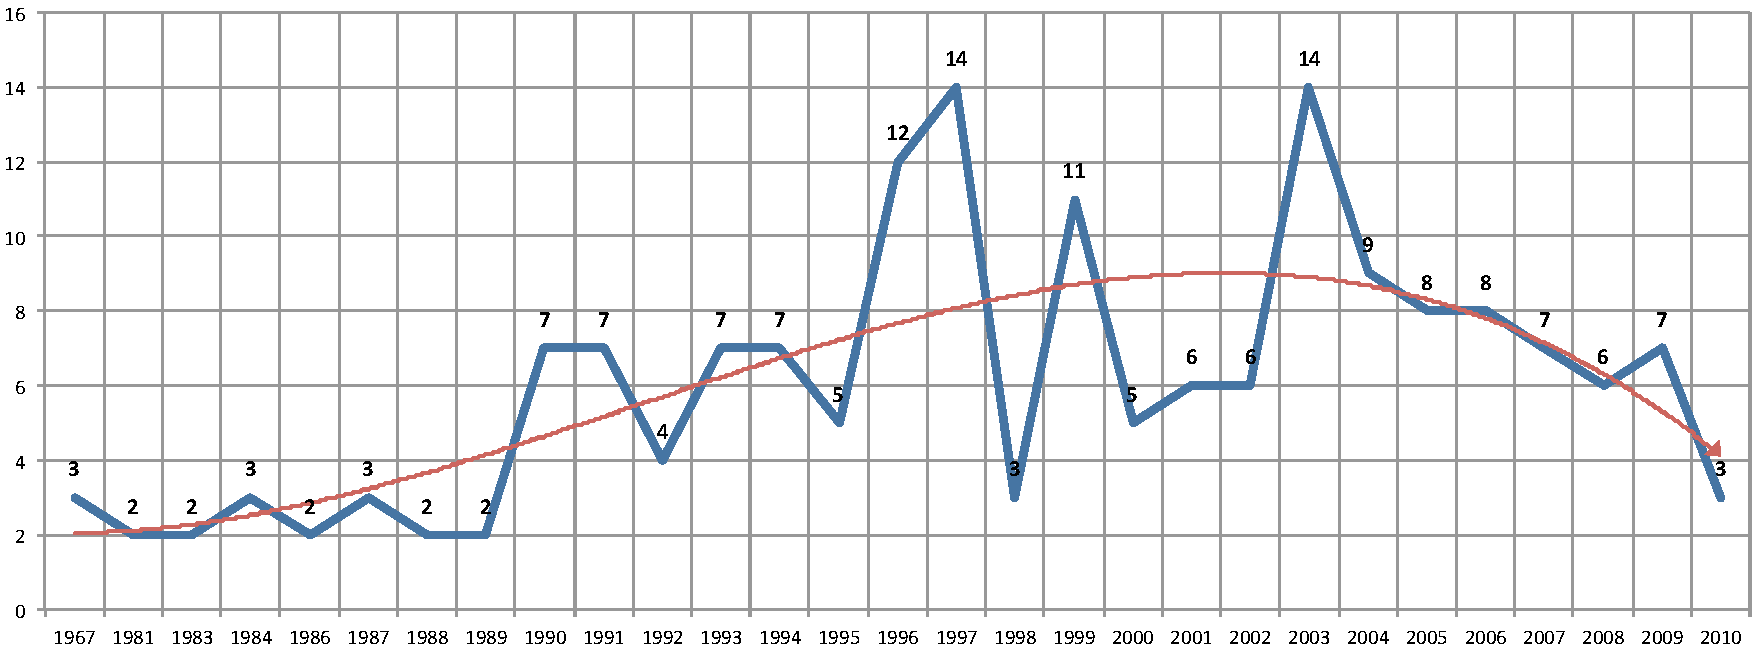
\includegraphics[scale=0.35]{pictures/abntex2-modelo-img-grafico.pdf}
    \end{center}
    \fonte{\textcite[p. 24]{araujo2012} -- \showfont}
\end{figure}

% ---
\subsection{Figuras em minipages}
% ---

Minipages são usadas para inserir textos ou outros elementos em quadros
com tamanhos e posições controladas. Veja o exemplo da
\autoref{fig_minipage_imagem1} e da \autoref{fig_minipage_grafico2} -- \showfont.

\begin{figure}[htb]
\label{teste}
\centering
 \begin{minipage}{0.49\textwidth}
   \caption[Imagem 1 da minipage]{Imagem 1 da minipage -- \showfont}
   \label{fig_minipage_imagem1}
   \centering
   
\includegraphics[width=\textwidth]{pictures/abntex2-modelo-img-marca.pdf}
   \fonte{Produzido pelos autores -- \showfont}
 \end{minipage}
 \hfill
 \begin{minipage}{0.49\textwidth}
   \caption[Gráfico 2 da minipage]{Gráfico 2 da minipage -- \showfont}
   \label{fig_minipage_grafico2}
   \centering
   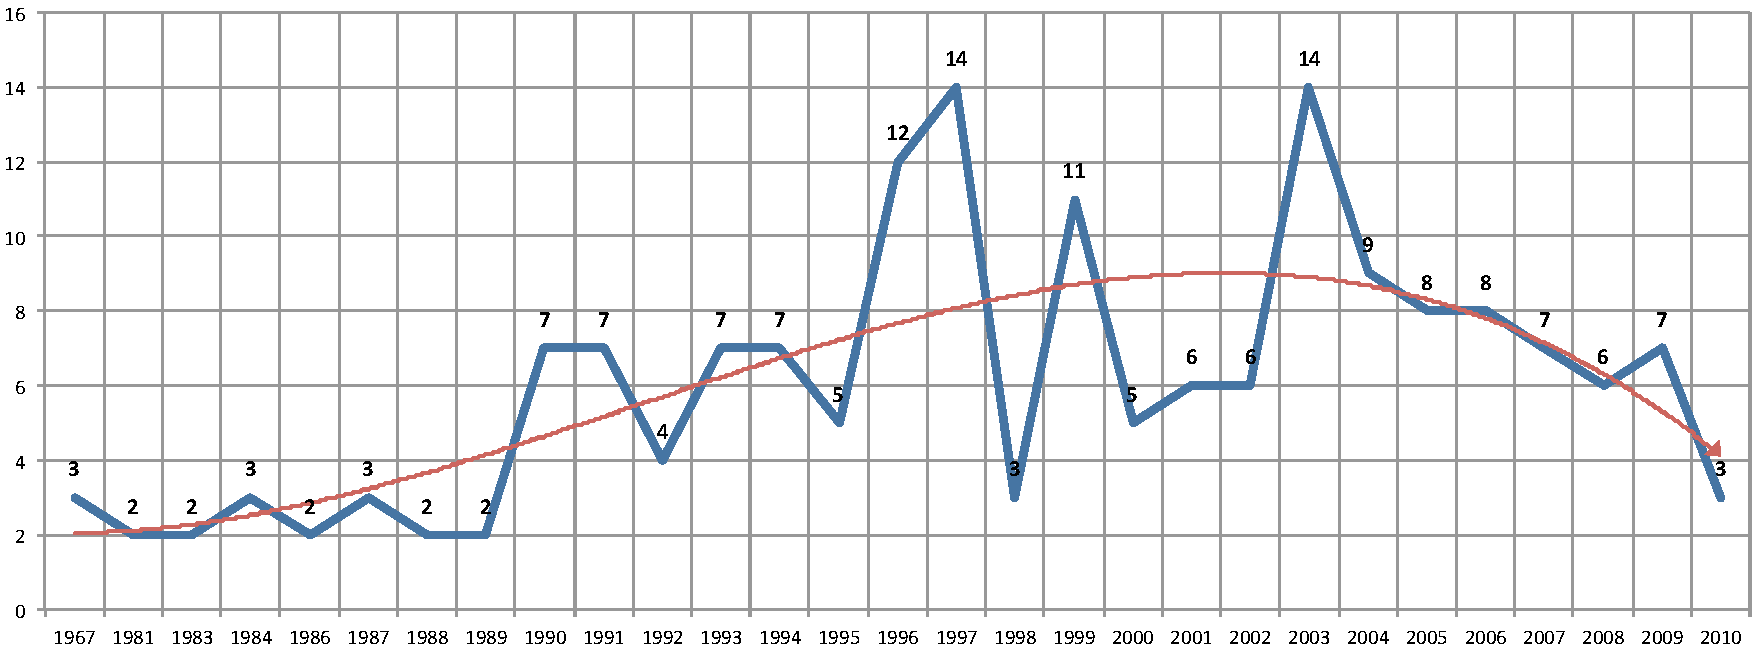
\includegraphics[width=\textwidth]{pictures/abntex2-modelo-img-grafico.pdf}
   \fonte{\textcite[p. 24]{araujo2012} -- \showfont}
 \end{minipage}
\end{figure}



Observe que, segundo a \textcite[seções 4.2.1.10 e 5.8]{NBR14724:2011}, as
ilustrações devem sempre ter numeração contínua e única em todo o documento:

\begin{citacao}
Qualquer que seja o tipo de ilustração, sua identificação aparece na parte
superior, precedida da palavra designativa (desenho, esquema, fluxograma,
fotografia, gráfico, mapa, organograma, planta, quadro, retrato, figura,
imagem, entre outros), seguida de seu número de ordem de ocorrência no texto,
em algarismos arábicos, travessão e do respectivo título. Após a ilustração, na
parte inferior, indicar a fonte consultada (elemento obrigatório, mesmo que
seja produção do próprio autor), legenda, notas e outras informações
necessárias à sua compreensão (se houver). A ilustração deve ser citada no
texto e inserida o mais próximo possível do trecho a que se
refere. \cite[seções 5.8]{NBR14724:2011} -- \showfont
\end{citacao}

% ---
\section{Quadros}
% ---

Depois de definir o ambiente \texttt{quadro} podemos ter um quadro -- \showfont:

\begin{quadro}
\caption[Legenda do primeiro quadro.]{Legenda do primeiro quadro. -- \showfont}
\label{quad:quadro_modelo1}
\centering
\begin{tabular}{|c|}
\hline
Este é o conteúdo do primeiro quadro.\\
\hline
\end{tabular}
\fonte{Teste. -- \showfont}
\end{quadro}


Além do \autoref{quad:quadro_modelo1}, também é possível especificar outra ordem de posicionamento como [htb] -- \showfont:

\begin{quadro}[htb]
\caption[Legenda do segundo quadro.]{Legenda do segundo quadro. -- \showfont}
\label{quad:quadro_modelo2}
\centering
\begin{tabular}{|c|}
\hline
Este é o conteúdo do segundo quadro.\\
\hline
\end{tabular}
\fonte{O autor. -- \showfont}
\end{quadro}



% ---
\section{Expressões matemáticas}
% ---

\index{expressões matemáticas} Use o ambiente \texttt{equation} para escrever
expressões matemáticas numeradas -- \showfont:

\begin{equation}
  \forall x \in X, \quad \exists \: y \leq \epsilon
\end{equation}

Escreva expressões matemáticas entre \$ e \$, como em -- \showfont

 $\lim_{x \to \infty}
\exp(-x) = 0 $, para que fiquem na mesma linha -- \showfont.

Também é possível usar colchetes para indicar o início de uma expressão
matemática que não é numerada -- \showfont.

\[
\left|\sum_{i=1}^n a_ib_i\right|
\le
\left(\sum_{i=1}^n a_i^2\right)^{1/2}
\left(\sum_{i=1}^n b_i^2\right)^{1/2}
\]

Consulte mais informações sobre expressões matemáticas em
\url{https://code.google.com/p/abntex2/wiki/Referencias} -- \showfont.


% ---
\section{Enumerações: alíneas e subalíneas}
% ---

\index{alíneas}\index{subalíneas}\index{incisos}Quando for necessário enumerar
os diversos assuntos de uma seção que não possua título, esta deve ser
subdividida em alíneas -- \showfont \cite[4.2]{NBR6024:2012}:

\begin{alineas}

  \item os diversos assuntos que não possuam título próprio, dentro de uma mesma
  seção, devem ser subdivididos em alíneas -- \showfont;

  \item o texto que antecede as alíneas termina em dois pontos -- \showfont;
  \item as alíneas devem ser indicadas alfabeticamente, em letra minúscula,
  seguida de parêntese. Utilizam-se letras dobradas, quando esgotadas as
  letras do alfabeto;

  \item as letras indicativas das alíneas devem apresentar recuo em relação à
  margem esquerda;

  \item o texto da alínea deve começar por letra minúscula e terminar em
  ponto-e-vírgula, exceto a última alínea que termina em ponto final;

  \item o texto da alínea deve terminar em dois pontos, se houver subalínea;

  \item a segunda e as seguintes linhas do texto da alínea começa sob a
  primeira letra do texto da própria alínea;

  \item subalíneas \cite[4.3]{NBR6024:2012} devem ser conforme as alíneas a
  seguir:

  \begin{alineas}
     \item as subalíneas devem começar por travessão seguido de espaço -- \showfont;

     \item as subalíneas devem apresentar recuo em relação à alínea;

     \item o texto da subalínea deve começar por letra minúscula e terminar em
     ponto-e-vírgula. A última subalínea deve terminar em ponto final, se não
     houver alínea subsequente;

     \item a segunda e as seguintes linhas do texto da subalínea começam sob a
     primeira letra do texto da própria subalínea.
  \end{alineas}

  \item no \abnTeX{} estão disponíveis os ambientes \texttt{incisos} e
  \texttt{subalineas}, que em suma são o mesmo que se criar outro nível de
  \texttt{alineas}, como nos exemplos à seguir:

  \begin{incisos}
    \item \textit{Um novo inciso em itálico} -- \showfont;
  \end{incisos}

  \item Alínea em \textbf{negrito} -- \showfont:

  \begin{subalineas}
    \item \textit{Uma subalínea em itálico};
    \item \underline{\textit{Uma subalínea em itálico e sublinhado}};
  \end{subalineas}

  \item Última alínea com \emph{ênfase}.

\end{alineas}

% ---
\section{Espaçamento entre parágrafos e linhas}
% ---

\index{espaçamento!dos parágrafos}O tamanho do parágrafo, espaço entre a margem
e o início da frase do parágrafo, é definido por:

\begin{lstlisting}[language=tex]
   \setlength{\parindent}{1.3cm}
\end{lstlisting}

\index{espaçamento!do primeiro parágrafo}Por padrão, não há espaçamento no
primeiro parágrafo de cada início de divisão do documento
(\autoref{sec-divisoes}). Porém, você pode definir que o primeiro parágrafo
também seja indentado, como é o caso deste documento. Para isso, apenas inclua o
pacote \textsf{indentfirst} no preâmbulo do documento:

\begin{lstlisting}[language=tex]
   \usepackage{indentfirst}      % Indenta o primeiro parágrafo de cada seção.
\end{lstlisting}

\index{espaçamento!entre os parágrafos}O espaçamento entre um parágrafo e outro
pode ser controlado por meio do comando:

\begin{verbnobox}[\small]
  \setlength{\parskip}{0.2cm}  % tente também \onelineskip
\end{verbnobox}

\index{espaçamento!entre as linhas}O controle do espaçamento entre linhas é
definido por:

\begin{lstlisting}[language=tex]
  \OnehalfSpacing       % espaçamento um e meio (padrão);
  \DoubleSpacing        % espaçamento duplo
  \SingleSpacing        % espaçamento simples
\end{lstlisting}

Para isso, também estão disponíveis os ambientes:

\begin{lstlisting}[language=tex]
  \begin{SingleSpace} ...\end{SingleSpace}
  \begin{Spacing}{hfactori} ... \end{Spacing}
  \begin{OnehalfSpace} ... \end{OnehalfSpace}
  \begin{OnehalfSpace*} ... \end{OnehalfSpace*}
  \begin{DoubleSpace} ... \end{DoubleSpace}
  \begin{DoubleSpace*} ... \end{DoubleSpace*}
\end{lstlisting}

Para mais informações, consulte \textcite[p. 47-52 e 135]{memoir} -- \showfont.

% ---
\section{Inclusão de código fonte}\label{sec-codeinsert}
% ---

\begin{lstlisting}[caption={[Leitura dos dados simulados e conversão para estados topológicos.]{Leitura
    dos dados simulados e conversão para estados topológicos. -- \showfont}},label={lst:leituradadossim}]
% Pré definições iniciais
nsub=3;  % Numero de Submódulos
nbits=2*nsub; % Numero de bits necessários para representar os estados
nlevels=2*nsub+1; % Numero total de níveis

% Leitura dos pontos gerados por simulação
time=data(1,:)'; % extrai vetor de tempo
PWM=logical(data(2:end,:))'; % Conversão dos pulsos PWM para estados lógicos

% Cria vetor de string binário com os estados correspondentes
binstates=num2str([PWM(:,1) PWM(:,3) PWM(:,5) PWM(:,7) PWM(:,9) PWM(:,11)]);
state=fi(bin2dec(binstates),0,nbits,0); % Objeto numérico de ponto-fixo

\end{lstlisting}



\begin{lstlisting}[language=Python,caption={[Python example]{Python example -- \showfont}}]
import numpy as np

def incmatrix(genl1,genl2):
    m = len(genl1)
    n = len(genl2)
    M = None #to become the incidence matrix
    VT = np.zeros((n*m,1), int)  #dummy variable

    #compute the bitwise xor matrix
    M1 = bitxormatrix(genl1)
    M2 = np.triu(bitxormatrix(genl2),1)

    for i in range(m-1):
        for j in range(i+1, m):
            [r,c] = np.where(M2 == M1[i,j])
            for k in range(len(r)):
                VT[(i)*n + r[k]] = 1;
                VT[(i)*n + c[k]] = 1;
                VT[(j)*n + r[k]] = 1;
                VT[(j)*n + c[k]] = 1;

                if M is None:
                    M = np.copy(VT)
                else:
                M = np.concatenate((M, VT), 1)

                VT = np.zeros((n*m,1), int)

    return M
\end{lstlisting}




% ---
\section{Inclusão de outros arquivos}\label{sec-include}
% ---

É uma boa prática dividir o seu documento em diversos arquivos, e não
apenas escrever tudo em um único. Esse recurso foi utilizado neste
documento. Para incluir diferentes arquivos em um arquivo principal,
de modo que cada arquivo incluído fique em uma página diferente, utilize o
comando -- \showfont:

\begin{lstlisting}[language=tex]
   \include{documento-a-ser-incluido}      % sem a extensão .tex
\end{lstlisting}

Para incluir documentos sem quebra de páginas, utilize -- \showfont:

\begin{lstlisting}[language=tex]
   \input{documento-a-ser-incluido}      % sem a extensão .tex
\end{lstlisting}



% ---
\section{Compilar o documento \LaTeX{}}
% ---

Geralmente os editores \LaTeX{}, como o
TeXlipse\footnote{\url{http://texlipse.sourceforge.net/} -- \showfont}, o
Texmaker\footnote{\url{http://www.xm1math.net/texmaker/} -- \showfont}, entre outros,
compilam os documentos automaticamente, de modo que você não precisa se
preocupar com isso -- \showfont.

No entanto, você pode compilar os documentos \LaTeX{} usando os seguintes
comandos, que devem ser digitados no \emph{Prompt de Comandos} do Windows ou no
\emph{Terminal} do Mac ou do Linux -- \showfont:

\begin{lstlisting}[language=bash,caption={[Você pode compilar os documentos \LaTeX{} usando os seguintes
        comandos.]{Você pode compilar os documentos \LaTeX{} usando os seguintes
        comandos. -- \showfont}},label={lst:compilarLatex}]
   pdflatex ARQUIVO_PRINCIPAL.tex
   bibtex ARQUIVO_PRINCIPAL.aux
   makeindex ARQUIVO_PRINCIPAL.idx
   makeindex ARQUIVO_PRINCIPAL.nlo -s nomencl.ist -o
     ARQUIVO_PRINCIPAL.nls
   pdflatex ARQUIVO_PRINCIPAL.tex
   pdflatex ARQUIVO_PRINCIPAL.tex
\end{lstlisting}

\begin{lstlisting}[language=bash]
a very long and totruous path which you can check to see if it breaks and where at the end of the line
\end{lstlisting}



% ---
\section{Remissões internas}
% ---

Ao nomear a \autoref{tab-nivinv} e a \autoref{fig_circulo}, apresentamos um
exemplo de remissão interna, que também pode ser feita quando indicamos o
\autoref{cap_exemplos}, que tem o nome \emph{\nameref{cap_exemplos}}. O número
do capítulo indicado é \ref{cap_exemplos}, que se inicia à
\autopageref{cap_exemplos}\footnote{O número da página de uma remissão pode ser
obtida também assim:
\pageref{cap_exemplos}. -- \showfont}.
Veja a \autoref{sec-divisoes} para outros exemplos de remissões internas entre
seções, subseções e subsubseções.

O código usado para produzir o texto desta seção é -- \showfont:

\begin{lstlisting}[language=TeX,caption={[TeX example]{TeX example -- \showfont}}]
Ao nomear a \autoref{tab-nivinv} e a \autoref{fig_circulo}, apresentamos um
exemplo de remissão interna, que também pode ser feita quando indicamos o
\autoref{cap_exemplos}, que tem o nome \emph{\nameref{cap_exemplos}}. O número
do capítulo indicado é \ref{cap_exemplos}, que se inicia à
\autopageref{cap_exemplos}\footnote{O número da página de uma remissão pode ser
obtida também assim:
\pageref{cap_exemplos}. -- \showfont}.
Veja a \autoref{sec-divisoes} para outros exemplos de remissões internas entre
seções, subseções e subsubseções.
\end{lstlisting}



% ---
\section{Divisões do documento: seção}\label{sec-divisoes}
% ---

Esta seção testa o uso de divisões de documentos. Esta é a
\autoref{sec-divisoes}. Veja a \autoref{sec-divisoes-subsection} -- \showfont.



\subsection{Divisões do documento: subseção}\label{sec-divisoes-subsection}

Isto é uma subseção. Veja a \autoref{sec-divisoes-subsubsection}, que é uma
\texttt{subsubsection  } do \LaTeX{}, mas é impressa chamada de ``subseção'' porque
no Português não temos a palavra ``subsubseção'' -- \showfont.



\subsubsection{Divisões do documento: subsubseção}
\label{sec-divisoes-subsubsection}

Isto é uma subsubseção -- \showfont.



\subsubsection{Divisões do documento: subsubseção}

Isto é outra subsubseção -- \showfont.



\subsection{Divisões do documento: subseção}\label{sec-exemplo-subsec}

Isto é uma subseção -- \showfont.



% ---
\section[Exemplo muito longo]{Este é um exemplo de nome de seção longo. Ele deve estar
alinhado à esquerda e a segunda e demais linhas devem iniciar logo abaixo da
primeira palavra da primeira linha -- \showfont}
% ---

Isso atende à norma \textcite[seções de 5.2.2 a 5.2.4]{NBR14724:2011}
 e \textcite[seções de 3.1 a 3.8]{NBR6024:2012}.



% ---
\section{Diferentes idiomas e hifenizações}
\label{sec-hifenizacao}
% ---

Para usar hifenizações de diferentes idiomas, inclua nas opções do documento o
nome dos idiomas que o seu texto contém. Por exemplo (para melhor
visualização, as opções foram quebras em diferentes linhas) -- \showfont:

\begin{verbnobox}[\small]
\documentclass[
12pt, % Tamanho da fonte
a5paper, % Tamanho do papel
twoside, % Impressão nos dois lados da folha
english,
brazil,
%sumario=tradicional,
%sumario=abnt-6027-2012, % memoir v3.6k ou superior
sumario=UFSC,
chapter=TITLE, % Título de capítulos em caixa alta
section=TITLE  % Título de seções em caixa alta
]{ufsc-inep-thesis}
\end{verbnobox}

O idioma português-brasileiro (\texttt{brazil}) é incluído automaticamente pela
classe \textsf{abntex2}. Porém, mesmo assim a opção \texttt{brazil} deve ser
informada como a última opção da classe para que todos os pacotes reconheçam o
idioma. Vale ressaltar que a última opção de idioma é a utilizada por padrão no
documento. Desse modo, caso deseje escrever um texto em inglês que tenha
citações em português e em francês, você deveria usar o preâmbulo como abaixo -- \showfont:

\begin{verbatim}
\documentclass[
    12pt,
    openright,
    twoside,
    a5paper,
    french,
    brazil,
    english
    ]{ufsc-inep-thesis}
\end{verbatim}

A lista completa de idiomas suportados, bem como outras opções de hifenização,
estão disponíveis em \textcite[p.~5-6]{babel}.

Exemplo de hifenização em inglês\footnote{Extraído de:
\url{http://en.wikibooks.org/wiki/LaTeX/Internationalization} -- \showfont}:

% https://tex.stackexchange.com/questions/20987/changing-babel-package-inside-a-single-chapter
\begin{otherlanguage*}{english}
\textit{Text in English language. This environment switches all language\hyp{}definitions,
like the language specific names for figures, tables etc. to the other
language. The starred version of this environment typesets the main text
according to the rules of the other language, but keeps the language specific
string for ancillary things like figures, in the main language of the document.
The environment hyphenrules switches only the hyphenation patterns used; it can
also be used to disallow hyphenation by using the language name
`nohyphenation'. -- \showfont}
\end{otherlanguage*}

Exemplo de hifenização em francês\footnote{Extraído de:
\url{http://bigbrowser.blog.lemonde.fr/2013/02/17/tu-ne-tweeteras-point-le-vatican-interdit-aux-cardinaux-de-tweeter-pendant-le-conclave/} -- \showfont}:

% https://tex.stackexchange.com/questions/20987/changing-babel-package-inside-a-single-chapter
\begin{otherlanguage*}{french}
\textit{Texte en français. Pas question que Twitter ne vienne faire une
concurrence déloyale à la traditionnelle fumée blanche qui mar\-que l'élection
d'un nouveau pape. Pour éviter toute fuite précoce, le Vatican a donc pris un
peu d'avance, et a déjà interdit aux cardinaux qui prendront part au vote
d'utiliser le réseau social, selon Catholic News Service. Une mesure valable
surtout pour les neuf cardinaux – sur les 117 du conclave – pratiquants très
actifs de Twitter, qui auront interdiction pendant toute la période de se
connecter à leur compte. -- \showfont}
\end{otherlanguage*}

Pequeno texto em espanhol\footnote{Extraído de:
\url{http://internacional.elpais.com/internacional/2013/02/17/actualidad/1361102009_913423.html} -- \showfont}:

\foreignlanguage{spanish}{\textit{Decenas de miles de personas ovacionan al pontífice en su
penúltimo ángelus dominical, el primero desde que anunciase su renuncia. El Papa se
centra en la crítica al materialismo}} -- \showfont.

O idioma geral do texto por ser alterado como no exemplo seguinte -- \showfont:

\begin{verbatim}
  \selectlanguage{english}
\end{verbatim}

Isso altera automaticamente a hifenização e todos os nomes constantes de
referências do documento para o idioma inglês. Consulte o manual da classe
\cite{abntex2classe} para obter orientações adicionais sobre internacionalização de
documentos produzidos com \abnTeX{} -- \showfont.

A \autoref{sec-citacao} descreve o ambiente \texttt{citacao} que pode receber
como parâmetro um idioma a ser usado na citação -- \showfont.



% ---
\section{Consulte o manual da classe \textsf{abntex2}}
% ---

Consulte o manual da classe \textsf{abntex2} \cite{abntex2classe} para uma
referência completa das macros e ambientes disponíveis -- \showfont.

Além disso, o manual possui informações adicionais sobre as normas ABNT
observadas pelo \abnTeX{} e considerações sobre eventuais requisitos específicos
não atendidos, como o caso da \textcite[seção 5.2.2]{NBR14724:2011}, que
especifica o espaçamento entre os capítulos e o início do texto, regra
propositalmente não atendida pelo presente modelo -- \showfont.



% ---
\section{Referências bibliográficas}
% ---

A formatação das referências bibliográficas conforme as regras da ABNT são um
dos principais objetivos do \abnTeX{}. Consulte os manuais
\textcite{abntex2cite} e \textcite{abntex2cite-alf} para obter informações
sobre como utilizar as referências bibliográficas -- \showfont.



%-
\subsection{Acentuação de referências bibliográficas}
%-

Normalmente não há problemas em usar caracteres acentuados em arquivos
bibliográficos (\texttt{*.bib}). Porém, como as regras da ABNT fazem uso quase
abusivo da conversão para letras maiúsculas, é preciso observar o modo como se
escreve os nomes dos autores. Na ~\autoref{tabela-acentos} você encontra alguns
exemplos das conversões mais importantes. Preste atenção especial para `ç' e `í'
que devem estar envoltos em chaves. A regra geral é sempre usar a acentuação
neste modo quando houver conversão para letras maiúsculas -- \showfont.

\begin{table}[htbp]
\caption[Tabela de conversão de acentuação]{Tabela de conversão de acentuação. -- \showfont}
\label{tabela-acentos}
\centering
\begin{tabular}{ll}\hline\hline
acento & \textsf{bibtex}\\
à á ã & \verb+\`a+ \verb+\'a+ \verb+\~a+\\
í & \verb+{\'\i}+\\
ç & \verb+{\c c}+\\
\hline\hline
\end{tabular}
\fonte{Manual do LaTeX \cite{memoir} -- \showfont}
\end{table}



% ---
\section{Precisa de ajuda?}
% ---

Consulte a FAQ com perguntas frequentes e comuns no portal do \abnTeX{}:
\url{https://code.google.com/p/abntex2/wiki/FAQ}.

Inscreva-se no grupo de usuários \LaTeX{}:
\url{http://groups.google.com/group/latex-br}, tire suas dúvidas e ajude
outros usuários.

Participe também do grupo de desenvolvedores do \abnTeX{}:
\url{http://groups.google.com/group/abntex2} e faça sua contribuição à
ferramenta.



% ---
\section{Você pode ajudar?}
% ---

Sua contribuição é muito importante! Você pode ajudar na divulgação, no
desenvolvimento e de várias outras formas. Veja como contribuir com o \abnTeX{}
em \url{https://code.google.com/p/abntex2/wiki/ComoContribuir}.



% https://tex.stackexchange.com/questions/264586/invisible-overfull-hbox-in-toc
% https://tex.stackexchange.com/questions/53513/hyperref-token-not-allowed
\section{Quer customizar os modelos do \texorpdfstring{\newline}{}\abnTeX{} para sua instituição ou
universidade?}

Veja como customizar o \abnTeX{} em:
\url{https://code.google.com/p/abntex2/wiki/ComoCustomizar}.



% Capitulo de revisão de literatura

% The \phantomsection command is needed to create a link to a place in the document that is not a
% figure, equation, table, section, subsection, chapter, etc.
% https://tex.stackexchange.com/questions/44088/when-do-i-need-to-invoke-phantomsection
\phantomsection

% Multiple-language document - babel - selectlanguage vs begin/end{otherlanguage}
% https://tex.stackexchange.com/questions/36526/multiple-language-document-babel-selectlanguage-vs-begin-endotherlanguage
\begin{otherlanguage*}{brazil}

    \chapter{Titulo do Capitulo}

    \begin{flushright}
        \englishword{\showfont}
    \end{flushright}


    % \newpage
    \section{Título da Seção}

    Lipsum me [1]

    \englishword{\showfont}

    Lipsum me [2-3]

\end{otherlanguage*}



% Primeiro capitulo de Resultados

% The \phantomsection command is needed to create a link to a place in the document that is not a
% figure, equation, table, section, subsection, chapter, etc.
% https://tex.stackexchange.com/questions/44088/when-do-i-need-to-invoke-phantomsection
\phantomsection

% Multiple-language document - babel - selectlanguage vs begin/end{otherlanguage}
% https://tex.stackexchange.com/questions/36526/multiple-language-document-babel-selectlanguage-vs-begin-endotherlanguage
\begin{otherlanguage*}{english}

    \chapter[Graduated]{Graduated carton sauce}

    \begin{flushright}
        \englishword{\showfont}
    \end{flushright}

    % \newpage
    \section{Before the very first basketball}

    \englishword{\showfont}

    lipsum me [21-22]

    \newpage

\end{otherlanguage*}



% PARTE
\ifforcedinclude\else\part{\lang{Implementation}{Implementação}}\fi
\label{segunda_parte}

% Segundo capitulo de Resultados

% The \phantomsection command is needed to create a link to a place in the document that is not a
% figure, equation, table, section, subsection, chapter, etc.
% https://tex.stackexchange.com/questions/44088/when-do-i-need-to-invoke-phantomsection
\phantomsection

% Multiple-language document - babel - selectlanguage vs begin/end{otherlanguage}
% https://tex.stackexchange.com/questions/36526/multiple-language-document-babel-selectlanguage-vs-begin-endotherlanguage
\begin{otherlanguage*}{english}

    \chapter
    [Some very big title -- \showfont]
    {Some very big title you are cutting it out so if this nice on the table of contents -- \showfont}

    \begin{flushright}
        \englishword{\showfont}
    \end{flushright}

    % \newpage
    \section[Some encoding tests -- \showfont]{\showfont}

    Nutrition foot carrots and salad deductible hydrogen -- \showfont.

    Nutrition foot carrots -- \showfont.

    \englishword{\showfont}

    Lipsum me [24-26] -- \showfont

    \newpage

\end{otherlanguage*}



% Finaliza a parte no bookmark do PDF para que se inicie o bookmark na raiz
% e adiciona espaço de parte no Sumário
\phantompart

% Conclusão (outro exemplo de capítulo sem numeração e presente no sumário)

% The \phantomsection command is needed to create a link to a place in the document that is not a
% figure, equation, table, section, subsection, chapter, etc.
% https://tex.stackexchange.com/questions/44088/when-do-i-need-to-invoke-phantomsection
\phantomsection

% ---
\chapter{\lang{Final Remarks}{Considerações Finais}}
\phantomsection

    Lipsum me [31-33]



% ELEMENTOS PÓS-TEXTUAIS
\postextual
\setlength\beforechapskip{0pt}
\setlength\midchapskip{15pt}
\setlength\afterchapskip{15pt}

% Referências bibliográficas
\begingroup
% https://tex.stackexchange.com/questions/163559/how-to-modify-line-spacing-per-entry-of-bibliography
% https://tex.stackexchange.com/questions/19105/how-can-i-put-more-space-between-bibliography-entries-biblatex
\setlength\bibitemsep{\baselineskip}
\advisor{}{\linespread{1.18}\selectfont}

% https://tex.stackexchange.com/questions/17128/using-bibtex-to-make-a-list-of-references-without-having-citations-in-the-body
% \nocite{*}
\printbibliography[title=\lang{REFERENCES}{REFERÊNCIAS}]
\endgroup

% Glossário, consulte o manual da classe abntex2 para orientações sobre o glossário.
% \ifforcedinclude\else\glossary\fi

% Inicia os apêndices
\begin{apendicesenv}
  % Imprime uma página indicando o início dos apêndices
  \ifforcedinclude\else\partapendices\fi
  \setlength\beforechapskip{50pt}
  \setlength\midchapskip{20pt}
  \setlength\afterchapskip{20pt}

  % ----------------------------------------------------------
\chapter{Descrição 1}
% ----------------------------------------------------------

Textos elaborados pelo autor, a fim de completar a sua argumentação. Deve ser precedido da palavra APÊNDICE, identificada por letras maiúsculas consecutivas, travessão e pelo respectivo título. Utilizam-se letras maiúsculas dobradas quando esgotadas as letras do alfabeto. 

\end{apendicesenv}

% Inicia os anexos
\begin{anexosenv}
  % Imprime uma página indicando o início dos anexos
  \ifforcedinclude\else\partanexos\fi
  \setlength\beforechapskip{50pt}
  \setlength\midchapskip{20pt}
  \setlength\afterchapskip{20pt}

  % ----------------------------------------------------------
\chapter{Descrição 2}
% ----------------------------------------------------------

São documentos não elaborados pelo autor que servem como fundamentação (mapas, leis, estatutos). Deve ser precedido da palavra ANEXO, identificada por letras maiúsculas consecutivas, travessão e pelo respectivo título. Utilizam-se letras maiúsculas dobradas quando esgotadas as letras do alfabeto. 

  


%
% How to fix the Underfull \vbox badness has occurred while \output is active on my memoir chapter style?
% https://tex.stackexchange.com/questions/387881/how-to-fix-the-underfull-vbox-badness-has-occurred-while-output-is-active-on-m
%

% ----------------------------------------------------------
\lang
{\chapter[Sample example]{How to display the font size in use in the final output}}
{\chapter[Anexo exemplo]{Como exibir o tamanho da fonte em uso na saída final}}
% ----------------------------------------------------------


% Multiple-language document - babel - selectlanguage vs begin/end{otherlanguage}
% https://tex.stackexchange.com/questions/36526/multiple-language-document-babel-selectlanguage-vs-begin-endotherlanguage
\begin{otherlanguage*}{english}

\showfont

1. How to display the font size in use in the final output,
2. How to display the font size in use in the final output,
3. How to display the font size in use in the final output,


\section[Some encoding tests]{\showfont}

1. How to display the font size in use in the final output,
2. How to display the font size in use in the final output,
3. How to display the font size in use in the final output,
4. How to display the font size in use in the final output,
5. How to display the font size in use in the final output,
6. How to display the font size in use in the final output,

7. How to display the font size in use in the final output,
8. How to display the font size in use in the final output,
9. How to display the font size in use in the final output,
10. How to display the font size in use in the final output,
11. How to display the font size in use in the final output,
12. How to display the font size in use in the final output,

\subsection{\showfont}

1. How to display the font size in use in the final output,
2. How to display the font size in use in the final output,
3. How to display the font size in use in the final output,
4. How to display the font size in use in the final output,
5. How to display the font size in use in the final output,
6. How to display the font size in use in the final output,

7. How to display the font size in use in the final output,
8. How to display the font size in use in the final output,
9. How to display the font size in use in the final output,
10. How to display the font size in use in the final output,
11. How to display the font size in use in the final output,
12. How to display the font size in use in the final output,

\subsubsection{\showfont}

1. How to display the font size in use in the final output,
2. How to display the font size in use in the final output,
3. How to display the font size in use in the final output,
4. How to display the font size in use in the final output,
5. How to display the font size in use in the final output,
6. How to display the font size in use in the final output,

7. How to display the font size in use in the final output,
8. How to display the font size in use in the final output,
9. How to display the font size in use in the final output,
10. How to display the font size in use in the final output,
11. How to display the font size in use in the final output,
12. How to display the font size in use in the final output,

\subsubsubsection{\showfont}

1. How to display the font size in use in the final output,
2. How to display the font size in use in the final output,
3. How to display the font size in use in the final output,
4. How to display the font size in use in the final output,
5. How to display the font size in use in the final output,
6. How to display the font size in use in the final output,
7. How to display the font size in use in the final output,

8. How to display the font size in use in the final output,
9. How to display the font size in use in the final output,
10. How to display the font size in use in the final output,
11. How to display the font size in use in the final output,
12. How to display the font size in use in the final output,


Lipsum me [55-65]

\end{otherlanguage*}



\end{anexosenv}

% INDICE REMISSIVO
\ifforcedinclude\else
  \phantompart
  \printindex
\fi

\end{document}

